%\documentclass[12pt]{article}

\questionheader{ex:sTF}

\begin{question}[M317 2013D] %8
True or false?
\begin{enumerate}[(a)]
\item
$\vnabla\cdot(\va \times\vr) = 0$, where $\va$ is a constant vector in 
$\bbbr^3$ , and $\vr$ is the vector field $\vr= (x, y, z)$.
\item
$\vnabla\times(\vnabla f) = 0$ for all scalar fields $f$ on $\bbbr^3$ 
with continuous second partial derivatives.
\item
$\vnabla\cdot(f \vF) = \vnabla(f)\cdot \vF + f \vnabla\cdot\vF$, 
for every vector field $\vF$ in $\bbbr^3$ with continuous partial derivatives, 
and every scalar function $f$ in $\bbbr^3$ with continuous partial
derivatives.
\item
Suppose $\vF$ is a vector field with continuous partial derivatives 
in the region $D$, where $D$ is $\bbbr^3$ without the origin. 
If $\vnabla\cdot\vF  > 0$ throughout $D$, then the flux of $F$ 
through the sphere of radius $5$ with center at the origin is positive.
%\item
%Suppose $\vF$ is a vector field with continuous partial derivatives 
%in all of $\bbbr^3$. Suppose further that $\vnabla\times\vF$
%has positive z-component everywhere in $\bbbr^3$. Then
%\begin{equation*}
%\int_0^\pi \vF \cdot (\cos \theta, \sin \theta, 0)\, \dee{\theta} 
% > \int_0^\pi \vF \cdot (\cos \theta, - \sin \theta, 0)\, \dee{\theta}
%\end{equation*}
\item
If a vector field $\vF$ is defined and has continuous partial 
derivatives everywhere in $\bbbr^3$, and it satisfies $\vnabla\cdot\vF = 0$, everywhere, then, for every sphere, the flux out of one hemisphere is equal 
to the flux into the opposite hemisphere.
\item
If $\vr(t)$ is a twice continuously differentiable path in $\bbbr^2$ 
with constant curvature $\kappa$, then $\vr(t)$ parametrizes part of a 
circle of radius $1/\kappa$.
\item
The vector field $\vF = \left( -\frac{y}{x^2+y^2}\,,\,\frac{x}{x^2+y^2}\right)$
is conservative in its domain, which is $\bbbr^2$, without the origin.
\item
If a vector field $\vF = (P, Q)$ in $\bbbr^2$ has $Q = 0$ everywhere in 
$\bbbr^2$, then the line integral $\oint\vF\cdot\dee{\vr}$ is zero, for every simple closed curve in $\bbbr^2$.
\item
If the acceleration and the speed of a moving particle in $\bbbr^3$ 
are constant, then the motion is taking place along a spiral.
\end{enumerate}
\end{question}

%\begin{hint} 
%
%\end{hint}

\begin{answer} 
(a) True\quad
(b) True\quad
(c) True\quad
(d) False\quad
%(e) True\quad
(e) True

(f) That depends. If $\ka=0$, the curve is part of a straight
line. If $\ka>0$ it is part of a circle of radius $\frac{1}{\ka}$.

(g) False.\quad
(h) False.\quad
(i) False.
\end{answer}

\begin{solution} (a) True.
For any constant vector $\va=(a_1,a_2,a_3)$,
\begin{align*}
\va\times\vr
&=\det\left[\begin{matrix}
\hi &\hj &\hk \\
a_1 & a_2 & a_3 \\
x   &  y  & z
\end{matrix}
\right]
= (a_2 z - a_3 y)\hi 
 -(a_1 z - a_3 x)\hj
 +(a_1 y - a_2 x)\hj
\end{align*}
This vector field does indeed have divergence $0$.

\noindent (b) True. This is our conservative field screening condition
Theorem \eref{CLP317}{thm:degTwoIdentities}.b.

\noindent (c) True. This is one of our vector identities, namely
Theorem \eref{CLP317}{thm:divIdentities}.c.

\noindent (d) False. The trap here is that $\vF$ need not be defined
at the origin. We saw, in Example \eref{CLP317}{eg:fluxIntegralA} of the CLP-4 text, that the point source $\vF_S=\frac{m\vr}{|\vr|^3}$ had flux 
$4\pi m$ through every sphere centred on the  origin. We also saw,
in Example \eref{CLP317}{eg:divThmD} of the CLP-4 text, that the divergence
$\vnabla\cdot\vF_S=0$ everywhere except at the origin (where it is not defined).
So if we choose $m$ to be a very big negative number (say $-10^{100}$)
and add in a very small vector field with positive divergence 
(say $ 10^{-100}(x\hi+y\hj +z\hk)$), we will get the vector field
$\vF = -10^{100}\frac{\vr}{|\vr|^3} + 10^{-100}(x\hi+y\hj +z\hk)$
which has divergence $\vnabla\cdot\vF=3\times 10^{-100}>0$ everywhere
except at the origin. The flux of this field through the specified sphere will
be $-4\pi\times 10^{100}$ plus a very small positive number. 

%\noindent (e) True. Denote
%\begin{align*}
%D&=\Set{(x,y,z)}{x^2+y^2\le 1,\ z=0} 
%             \text{ with normal $\hk$}\\
%C_+&=\Set{(x,y,z)}{x^2+y^2= 1,\ z=0,\ y\ge 0} 
%            \text{ oriented counterclockwise}\\
%C_-&=\Set{(x,y,z)}{x^2+y^2= 1,\ z=0,\ y\le 0} 
%            \text{ oriented clockwise}
%\end{align*}
%Then
%\begin{equation*}
%\int_0^\pi \vF \cdot (\cos \theta, \sin \theta, 0)\, \dee{\theta} 
%     =\int_{C_+}\vF\cdot\dee{\vr}\qquad
%\int_0^\pi \vF \cdot (\cos \theta, - \sin \theta, 0)\, \dee{\theta}
%     =\int_{C_-}\vF\cdot\dee{\vr}
%\end{equation*}
%and, by Stokes' theorem,
%\begin{align*}
%\int_{C_+}\vF\cdot\dee{\vr} - \int_{C_-}\vF\cdot\dee{\vr}
%=\int_{\partial D}\vF\cdot\dee{\vr}
%=\dblInt_{D}\vnabla\times \vF\cdot \hk\, \dee{S}
%>0
%\end{align*}

\noindent (e) True. The statement that 
 ``the flux out of one hemisphere is equal 
   to the flux into the opposite hemisphere''
is equivalent to the statement that
  ``the flux out of the sphere is equal to zero''.
Since $\vnabla\cdot\vF=0$ everywhere, that is true by the divergence
theorem.

\noindent (f) That depends. 

If $\ka=0$, then $\diff{\hat\vT}{s}=0$, so that $\diff{\vr}{s}=\hat\vT$
is a constant. So $\vr(s) = s\hat\vT +\vr(0)$ is part of a straight line.

If $\ka>0$, then, because the curve is in a plane, the torsion $\tau$ is
zero and the Frenet-Serret formulae reduce to
\begin{equation*}
\diff{\hat\vT}{s} = \ka\hat\vN\qquad
\diff{\hat\vN}{s} = -\ka\hat\vT
\end{equation*}
Now consider the centre of curvature $\vc(s) = \vr(s) +\frac{1}{\ka}\hat\vN(s)$.
Since 
\begin{equation*}
\diff{\vc}{s} = \diff{\vr}{s} +\frac{1}{\ka}\diff{\hat\vN}{s}
              =\hat\vT(s) +\frac{1}{\ka}\big(-\ka\hat\vT(s)\big)
              =\vZero
\end{equation*}
$\vc(s)$ is a constant and
\begin{equation*}
|\vr(s) -\vc| =\frac{1}{\ka}
\end{equation*}
which says that the curve is part of the circle of radius $\frac{1}{\ka}$
centred on $\vc$.

\noindent (g) False. We saw in Examples 
\eref{CLP317}{eg:screeningCounterexample} and
\eref{CLP317}{eg:greenCC} of the CLP-4 text that the given vector 
field is not conservative. 

\noindent (h) False. For example, if $P=-y$, then 
$\oint_C\vF\cdot\dee{\vr}=-\oint_C y\,\dee{x}$
is the area inside $C$. See Corollary \eref{CLP317}{cor:greens}
in the CLP-4 text.

\noindent (i) False. 

If $\diff{\vv}{t}=\va$ is a constant, then
$\vv(t) =\va\, t+\vv_0$. Integrating a second time,
$\vr(t) = \frac{1}{2}\va\,t^2 +\vv_0\, t+\vr_0$. This is not a spiral,
whether or not the speed is constant. (In fact, for the speed $|\vv(t)|
=|\va\, t+\vv_0|$ to be constant, $\va$ has to be $\vZero$,
so that $\vr(t) = \vv_0\, t+\vr_0$ is a straight line.)

Another way to come to the same conclusion uses
\begin{equation*}
\va(t)=\difftwo{s}{t}(t)\,\hat\vT(t)
                             +\ka(t)\Big(\diff{s}{t}(t)\Big)^2\hat\vN(t)
\end{equation*}
As the speed $\diff{s}{t}$ is a constant, it reduces to 
\begin{equation*}
\va(t)=\ka(t)\Big(\diff{s}{t}(t)\Big)^2\hat\vN(t)
\end{equation*}
As $\va(t)$ is a constant, its direction, $\hat\vN(t)$, is also
a constant. The normal vector to a spiral is not constant.
\end{solution}
%%%%%%%%%%%%%%%%%%%%%%%%%%%

\goodbreak
\begin{question}[M317 2012D] %8
True or false?
\begin{enumerate}[(a)]
\item
$\vnabla\times(\va \times\vr) = 0$, where $\va$ is a constant vector in 
$\bbbr^3$ , and $\vr$ is the vector field $\vr= (x, y, z)$.
\item
$\vnabla\cdot(\vnabla f) = 0$ for all scalar fields $f$ on $\bbbr^3$ 
with continuous second partial derivatives.
\item
$\vnabla(\vnabla\cdot \vF) = 0$ for every vector field $\vF$ on $\bbbr^3$ 
with continuous second partial derivatives.
\item
Suppose $\vF$ is a vector field with continuous partial derivatives 
in the region $D$, where $D$ is $\bbbr^3$ without the origin.  If $\vnabla\cdot\vF = 0$,  then the flux of $\vF$ through
the sphere of radius $5$ with center at the origin is $0$.
\item
Suppose $\vF$ is a vector field with continuous partial derivatives 
in the region $D$, where $D$ is $\bbbr^3$ without the origin. If 
$\vnabla\times\vF=\vZero$ then  $\oint_C\vF\cdot\dee{\vr}$ is zero, for 
every simple and smooth closed curve $C$ in $\bbbr^3$ which avoids the origin.
\item
If a vector field $\vF$ is defined and has continuous partial 
derivatives everywhere in $\bbbr^3$, and it satisfies $\vnabla\cdot\vF > 0$, everywhere, then, for every sphere, the flux \emph{out} of one hemisphere 
is larger than  the flux \emph{into} the opposite hemisphere.
\item
If $\vr(t)$ is a path in $\bbbr^3$ 
with constant curvature $\kappa$, then $\vr(t)$ parametrizes part of a 
circle of radius $1/\kappa$.
\item
The vector field $\vF = \left( -\frac{y}{x^2+y^2}\,,\,\frac{x}{x^2+y^2}
\,,\,z\right)$
is conservative in its domain, which is $\bbbr^3$, without the $z$-axis.
\item
If all flow lines of a vector field in $\bbbr^3$ are parallel to the 
$z$-axis, then the circulation of the vector field around every closed 
curve is $0$.
\item
If the speed of a moving particle is constant, then its acceleration 
is orthogonal to its velocity.
\end{enumerate}
\end{question}

\begin{hint} 
Read (d), (e), (f), (g), (h) very carefully.
\end{hint}

\begin{answer} 
(a) False\qquad
(b) False\qquad
(c) False\qquad
(d) False\qquad
(e) True\qquad
(f) True

(g) False\qquad
(h) False\qquad
(i) False\qquad
(j) True
\end{answer}

\begin{solution} (a)
False.
For any constant vector $\va=(a_1,a_2,a_3)$,
\begin{align*}
\va\times\vr
&=\det\left[\begin{matrix}
\hi &\hj &\hk \\
a_1 & a_2 & a_3 \\
x   &  y  & z
\end{matrix}
\right]
= (a_2 z - a_3 y)\hi 
 -(a_1 z - a_3 x)\hj
 +(a_1 y - a_2 x)\hj
\end{align*}
So 
\begin{align*}
\vnabla\times(\va\times\vr)
&=\det\left[\begin{matrix}
\hi &\hj &\hk \\
\tfrac{\partial\hfill}{\partial x} & \tfrac{\partial\hfill}{\partial y} & 
                \tfrac{\partial\hfill}{\partial z} \\
a_2 z - a_3 y & -a_1 z + a_3 x & a_1 y - a_2 x
\end{matrix}
\right]
=2 a_1\hi + 2 a_2\hj + 2 a_3\hk 
\end{align*}
is nonzero, unless the constant vector $\va=\vZero$.

\noindent (b)
False. For example, if $f(x) = x^2$, then
\begin{align*}
\vnabla\cdot(\vnabla f)
=\vnabla\cdot(\vnabla x^2)
=\vnabla\cdot(2x\hi)
=2
\end{align*}

\noindent (c)
False. For example, if $\vF = x^2\hi$, then
\begin{align*}
\vnabla(\vnabla\cdot\vF)
=\vnabla\big(\vnabla\cdot(x^2\hi)\big)
=\vnabla(2x)
=2\hi
\end{align*}

\noindent (d)
False. The trap here is that $\vF$ need not be defined
at the origin. We saw, in Example \eref{CLP317}{eg:fluxIntegralA} of the CLP-4
text, that the point source $\vF=\frac{m\vr}{|\vr|^3}$ had flux 
$4\pi m$ through every sphere centred on the  origin. We also saw,
in Example \eref{CLP317}{eg:divThmD} of the CLP-4 text, that the divergence
$\vnabla\cdot\vF=0$ everywhere except at the origin (where it is not defined).


\noindent (e)
True. Any simple, smooth, closed curve in $\bbbr^3$ that avoids the origin
is the boundary of a surface $S$ that also avoids the origin. Then,
by Stokes' theorem,
\begin{equation*}
\oint_C\vF\cdot\dee{\vr} 
=\dblInt_S \vnabla\times\vF\cdot\hn\,\dee{S}
=0
\end{equation*}

\noindent (f)
True. Let $S=\Set{\vr}{|\vr-\vc|=R}$ be a sphere. 
Denote by $V=\Set{\vr}{|\vr-\vc|\le R}$ the ball whose boundary is $S$.
Let $H$ be one hemisphere of $S$ with outward pointing normal and let 
$H'$ be the other hemisphere of $S$ with inward
point normal. Then the boundary of $V$, with outward pointing normal,
can be viewed as consisting of two parts, namely $H$ and $-H'$,
where by $-H'$ we mean $H'$ but with outward pointing normal. 
Then, by the divergence theorem
\begin{align*}
\dblInt_H \vF\cdot\hn\,\dee{S} - 
\dblInt_{H'} \vF\cdot\hn\,\dee{S}
&=\dblInt_{\partial V} \vF\cdot\hn\,\dee{S} \\
&=\tripInt_V \vnabla\cdot\vF\,\dee{V}>0
\end{align*} 
which implies that $\dblInt_H \vF\cdot\hn\,\dee{S} > 
\dblInt_{H'} \vF\cdot\hn\,\dee{S}$.

\noindent (g)
False. The trap here is that the curve is in $\bbbr^3$, not $\bbbr^2$. 
As we saw in Example \eref{CLP317}{eg:helixTwist} of the CLP-4 text, 
a helix has constant curvature, but does not lie in a plane and so 
is not part of a circle. 

\noindent (h)
False. Even if we restrict $\vF$ to the $xy$-plane (i.e. to $z=0$), 
this vector field is not conservative. We saw that in Examples 
\eref{CLP317}{eg:screeningCounterexample} and
\eref{CLP317}{eg:greenCC} of the CLP-4 text.

\noindent (i)
False. For example, the vector field $\vF = x\,\hk$ is always parallel to the 
$z$-axis. So its flow lines are also all parallel to the $z$-axis.
But if the closed curve $C$ consists of the line segments
\begin{itemize}\itemsep1pt \parskip0pt \parsep0pt %\itemindent-15pt
\item[$\circ$]
$L_1$ from $(0,0,0)$ to $(1,0,0)$, followed by
\item[$\circ$]
$L_2$ from $(1,0,0)$ to $(1,0,1)$, followed by
\item[$\circ$]
$L_3$ from $(1,0,1)$ to $(0,0,1)$, followed by
\item[$\circ$]
$L_4$ from $(0,0,1)$ back to $(0,0,0)$,
\hskip1.0in
\raisebox{-25pt}[0pt][5pt]{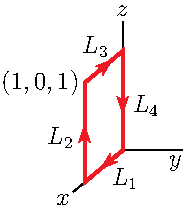
\includegraphics{OE12D_8h.pdf}}
\end{itemize} 
then
\begin{itemize}\itemsep1pt \parskip0pt \parsep0pt %\itemindent-15pt
\item[$\circ$]
$\int_{L_1} \vF\cdot\dee{\vr} = \int_0^1 (x\hk)\cdot\hi\,\dee{x} = 0$
since $\hk\perp\hi$, $\dee{\vr}=\hi\,\dee{x}$ on $L_1$ and
\item[$\circ$]
$\int_{L_2} \vF\cdot\dee{\vr} = \int_0^1 (1\hk)\cdot\hk\,\dee{z} = 1$
since $x=1$ and $\dee{\vr}=\hk\,\dee{z}$ on $L_2$ and
\item[$\circ$]
$\int_{L_3} \vF\cdot\dee{\vr} = -\int_0^1 (x\hk)\cdot\hi\,\dee{x} = 0$
since $\hk\perp\hi$ and
\item[$\circ$]
$\int_{L_4} \vF\cdot\dee{\vr} = -\int_0^1 (0\hk)\cdot\hk\,\dee{z} = 0$
since $x=0$ on $L_4$.
\end{itemize} 
All together
\begin{equation*}
\int_{C} \vF\cdot\dee{\vr}
=\int_{L_1} \vF\cdot\dee{\vr}
+\int_{L_2} \vF\cdot\dee{\vr}
+\int_{L_3} \vF\cdot\dee{\vr}
+\int_{L_4} \vF\cdot\dee{\vr}
=1
\end{equation*}


\noindent (j) 
True. If the speed $|\vv|$ is constant then
\begin{align*}
0= \diff{\hfill}{t} |\vv|^2
= \diff{\hfill}{t} (\vv\cdot\vv)
= 2\vv\cdot\va
\end{align*}


\end{solution}

%%%%%%%%%%%%%%%%%%%%%%%%%%%%

\begin{question}[M317 2011D]  %1

\begin{enumerate}[(a)]
\item
True or false? If $\vr(t)$ is the position at time $t$ of an object moving 
in $\bbbr^3$, and $\vr(t)$ is twice differentiable, then $|\vr''(t)|$ is 
the tangential component of its acceleration.

\item
Let $\vr(t)$ is a smooth curve in $\bbbr^3$ with unit tangent, normal 
and binormal vectors $\hat\vT(t)$, $\hat\vN(t)$, $\hat\vB(t)$. Which two of these 
vectors span the plane normal to the curve at $\vr(t)$?

\item
True or false? If $\vF = P\hi + Q\hj + R\hk$ is a vector field on 
$\bbbr^3$ such that $P$, $Q$, $R$ have continuous first order derivatives, 
and if $\vnabla\times\vF = \vZero$ everywhere on $\bbbr^3$ , then $\vF$ 
is conservative.

\item
True or false? If $\vF = P\hi + Q\hj + R\hk$  is a vector field on 
$\bbbr^3$ such that $P$, $Q$, $R$ have continuous second order derivatives, 
then $\vnabla\times(\vnabla\cdot F) = 0$.

\item
True or false? If $\vF$ is a vector field on $\bbbr^3$ such that 
$|\vF(x, y, z)| = 1$ for all $x$, $y$, $z$, and
if $S$ is the sphere $x^2 + y^2 + z^2 = 1$, then 
$\dblInt_S \vF \cdot\hn\,\dee{S} = 4\pi$.

\item
True or false? Every closed surface $S$ in $\bbbr^3$ is orientable. 
(Recall that $S$ is closed if it is the boundary of a solid region $E$.)

\end{enumerate}
\end{question}

\begin{hint} 
Beware that in part (f) a surface is defined to be closed if and only if it is
the boundary of a solid region $E$. Even though that is not the usual 
definition, it is be used in this question. 
\end{hint}

\begin{answer} 
(a) False.\qquad
(b) $\hat\vN(t)$, $\hat\vB(t)$\qquad
(c) True.\qquad
(d) False.\qquad
(e) False.\qquad
(f) True.

\end{answer}

\begin{solution} (a)
False. $\vr''(t)$ is the full acceleration. So $|\vr''(t)|$
is the magnitude of the full acceleration, not just the tangential
component of acceleration. For example, if $\vr(t) =\cos t\,\hi+\sin t\,\hj$
(i.e. the particle is just going around in circles), the
acceleration $\vr''(t) = -\cos t\,\hi-\sin t\,\hj$ is perpendicular
to the direction of motion. So the tangential component of acceleration
is zero, while $|\vr''(t)|=1$.

\noindent (b) $\hat\vT(t)$ is the tangent vector to the curve at $\vr(t)$.
$\hat\vN(t)$ and $\hat\vB(t)$ are both perpendicular to $\hat\vT(t)$
(and to each other) and so span the plane normal to the curve at $\vr(t)$.

\noindent (c) True.
This is (half of) Theorem  \eref{CLP317}{thm:screenConserv} in
the CLP-4 text.

\noindent (d) False. The statement $\vnabla\times(\vnabla\cdot F) = 0$
is just plain gibberish, because $\vnabla\cdot F$ is a scalar valued function
and there is no such thing as the curl of a scalar valued function.

\noindent (e) False. For example if $\vF=\hi$, then, by the divergence theorem,
\begin{equation*}
\dblInt_S \vF \cdot\hn\,\dee{S} 
 =\tripInt_V\vnabla\cdot\vF\,\dee{V}=0
\end{equation*}
Here $V=\Set{x,y,z}{x^2+y^2+z^2\le 1}$ is the inside of the sphere.

\noindent (f) True. If $S$ is the boundary of the solid region $E$, then
we can orient $S$ by always choosing the normal vector that points into $E$. 

\end{solution}

\goodbreak
%%%%%%%%%%%%%%%%%%%%%%%%%%%
\begin{question}[M317 2010D] %9

\begin{enumerate}[(a)]
\item
In the curve shown below (a helix lying in the surface of a cone), is the
curvature increasing, decreasing, or constant as z increases?

\begin{center}
       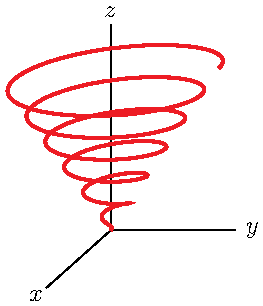
\includegraphics{helixCone.pdf}
\end{center}

%Circle the answer:\quad
%increasing\quad
%decreasing\quad
%constant

\item
Of the two functions shown below, one is a function $f(x)$ and one is its
curvature $\kappa(x)$. Which is which?

\begin{center}
       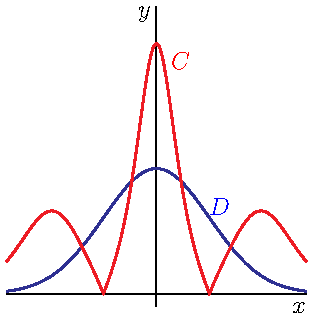
\includegraphics{OE10D_10b.pdf}
\end{center}


%$f(x)$ is (circle one):\quad
%C\quad
%D

\item
Let $C$ be the curve of intersection of the cylinder $x^2 + z^2 = 1$ 
and the saddle $xz = y$. Parametrise $C$. (Be sure to specify the domain of
your parametrisation.)

\item 
Let $H$ be the helical ramp (also known as a helicoid) which revolves around
the $z$-axis in a clockwise direction viewed from above, beginning 
at the y-axis when $z = 0$, and rising $2\pi$ units each time it makes 
a full revolution. Let $S$ be the portion
of $H$ which lies outside the cylinder $x^2 + y^2 = 4$, above the 
$z = 0$ plane and below the $z = 5$ plane.
Choose one of the following functions and give the domain on which the 
function you have chosen parametrizes S. (Hint: Only one of the following functions is possible.)
\begin{enumerate}[(a)]
\item 
$\vr(u, v) = \big(u \cos v, u \sin v, u\big)$
\item 
$\vr(u, v) = \big(u \cos v, u \sin v, v\big)$
\item 
$\vr(u, v) = \big(u \sin v, u \cos v, u\big)$
\item 
$\vr(u, v) = \big(u \sin v, u \cos v, v\big)$
\end{enumerate}

\item 
Write down a parametrized curve of zero curvature and arclength $1$.
(Be sure to specify the domain of your parametrisation.)

\item 
If $\vnabla\cdot\vF$ is a constant $C$ on all of $\bbbr^3$, and 
$S$ is a cube of unit volume such that the flux outward through each 
side of $S$ is $1$, what is $C$?

\item
Let
\begin{equation*}
\vF(x, y) = \big(ax + by\,,\, cx + dy\big)
\end{equation*}
Give the full set of $a$, $b$, $c$ and $d$ such that $\vF$ is conservative.

\item 
If $\vr(s)$ has been parametrized by arclength (i.e. $s$ is arclength), 
what is the arclength of $\vr(s)$ between $s = 3$ and $s = 5$?

\item 
Let $\vF$ be a 2D vector field which is defined everywhere except at 
the points marked $P$ and $Q$. Suppose that $\vnabla\times\vF = 0$ 
everywhere on the domain of $\vF$. Consider
the five curves $R$, $S$, $T$, $U$, and $V$ shown in the picture. 

  \begin{center}
       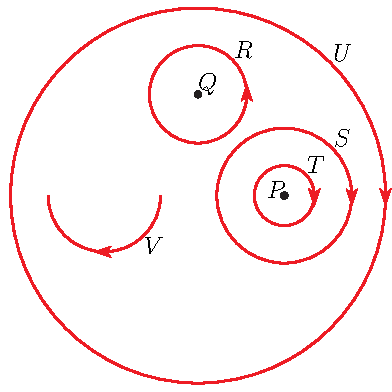
\includegraphics[scale=0.8]{OE10D_10i.pdf}
  \end{center}

Which of the following is necessarily true?
\begin{enumerate}[(1)]
\item $\int_S \vF\cdot\dee{\vr} = \int_T \vF\cdot\dee{\vr}$

\item $\int_R \vF\cdot\dee{\vr} = \int_S \vF\cdot\dee{\vr} 
 = \int_T \vF\cdot\dee{\vr} = \int_U \vF\cdot\dee{\vr} = 0$

\item $\int_R \vF\cdot\dee{\vr} + \int_S \vF\cdot\dee{\vr} 
       + \int_T \vF\cdot\dee{\vr} = \int_U \vF\cdot\dee{\vr}$

\item $\int_U \vF\cdot\dee{\vr} = \int_R \vF\cdot\dee{\vr} 
   + \int_S \vF\cdot\dee{\vr}$

\item $\int_V \vF\cdot\dee{\vr} = 0$
\end{enumerate}

\item 
Write down a 3D vector field $\vF$ such that for all closed surfaces $S$, 
the volume enclosed by $S$ is equal to
\begin{equation*}
\dblInt_S \vF \cdot \hn\,\dee{S}
\end{equation*}

\item 
Consider the vector field $\vF$ in the $xy$-plane shown below.
Is the $\hk^{\rm th}$ component of $\vnabla\times\vF$ at $P$ 
positive, negative or zero?

  \begin{center}
       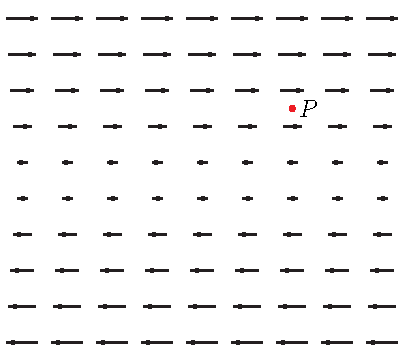
\includegraphics[scale=0.8]{shearField.pdf}
  \end{center}





\end{enumerate}
\end{question}

\begin{hint} 
(b) In general, for which values of $x$ is the curvature of $y=f(x)$ zero?

(c) First parametrize $x^2+z^2=1$.

(d) First determine when $\vr(u,v)$ has $z=0$. 

(e) What type of curve has curvature zero?

(f) What theorem relates the divergence of a vector field with flux
integrals of the vector field? 

(g) What is the screening test for conservativeness in two dimensions?

(h) What is the definition of ``parametrized by arclength''?

(i) What theorem relates line integrals to curls?

(j) What theorem relates flux integrals to divergences?

(k) Use Stokes' theorem.


\end{hint}

\begin{answer} 
(a) decreasing\qquad
(b) $f(x)$ is $D$

(c) $\vr(\theta) = \cos\theta\,\hi +\sin\theta\,\hk 
         + \sin\theta\,\cos\theta\,\hj$,  $0\le\theta<2\pi$

(d) We want parametrisation (d) with domain $|u|\ge 2$, $0\le v\le 5$.

(e) One possible answer is $\vr(t) = t\,\hi$, $0\le t\le 1$.

(f) $C=6$\qquad
(g) $\Set{(a,b,c,d)}{a,b,c,d\text{ all real and }b=c}$\qquad
(h) 2

(i) (1) True \quad
    (2) False \quad
    (3) False \quad
    (4) False \quad
    (5) False

(j) Any vector field whose divergence is $1$ everywhere will work.
One such vector field is $\vF=x\,\hi$.

(k) negative

\end{answer}



\begin{solution}  (a) The helix is approximately a bunch of circles
stacked one on top of each other. The radius of the circles increase
as $z$ increases. So the curvature \emph{decreases} as $z$ increases.

\noindent (b) Here are two arguments both of which conclude that $f(x)$
is $D$. 

\begin{itemize}\itemsep1pt \parskip0pt \parsep0pt %\itemindent-15pt
\item[$\circ$] If $C$ were the graph $y=f(x)$, then $f'(x)$ would
have two points of discontinuity. The curvature $\ka(x)$ would not the
defined at those two points. The function whose graph is $D$ is defined
everywhere and so cannot be the curvature of the function whose graph is $C$. 

\item[$\circ$] The function whose graph is $D$ has two inflection points.
So its curvature is zero at two points. The function whose graph is $C$
is indeed zero at two points (that in fact correspond to the inflection points
of $D$). So $D$ is the graph of $f(x)$ and $C$ is the graph of $\kappa(x)$.
\end{itemize} 

\noindent (c) For any fixed $y$, $x^2+z^2=1$ is a circle of radius $1$.
So we can parametrize it by $x(\theta)=\cos\theta$, 
$z(\theta)=\sin\theta$, $0\le\theta<2\pi$. The $y$-coordinate of any point on
the intersection is determined by $y=xz$. So we can use
\begin{equation*}
\vr(\theta) = \cos\theta\,\hi +\sin\theta\,\hk + \sin\theta\,\cos\theta\,\hj
\qquad 0\le\theta<2\pi
\end{equation*}

\noindent (d)
We are told that the helical ramp starts starts with the $y$-axis when
$z=0$.
\begin{itemize}\itemsep1pt \parskip0pt \parsep0pt %\itemindent-15pt
\item[$\circ$] 
In the cases of parametrisations (a) and (c),
$z=0$ forces $u=0$ and $u=0$ forces $x=y=0$. That is only the
origin, not the $y$-axis. So we can rule out (a) and(c).

\item[$\circ$] 
In the case of parametrisation (b), 
$z=0$ forces $v=0$ and $v=0$ forces $y=0$ and $x=u$. As $u$ varies 
that sweeps out the $x$-axis, not the $y$-axis. 
So we can rule out (b).

\item[$\circ$] 
In the case of parametrisation (d), 
$z=0$ forces $v=0$ and $v=0$ forces $x=0$ and $y=u$. As $u$ varies 
that sweeps out the $y$-axis, which is what we want.
\end{itemize} 
Furthermore
\begin{itemize}\itemsep1pt \parskip0pt \parsep0pt %\itemindent-15pt
\item[$\circ$] 
we are told that $z=v$ runs from $0$ to $5$ and that
\item[$\circ$] 
$x^2+y^2=u^2\ge 4$
\end{itemize} 
So we want parametrisation (d) with domain $|u|\ge 2$, $0\le v\le 5$.

\noindent (e) 
Straight lines have curvature $0$. So one acceptable
parametrized curve is $\vr(t) = t\,\hi$, $0\le t\le 1$.

\noindent (f) 
The cube $S$ has six sides. So the outward flux through
$\partial S$ is $6$ and, by the divergence theorem,
\begin{align*}
6 &= \dblInt_{\partial S}\vF\cdot\hn\,\dee{S}
   =\tripInt_S \vnabla\cdot\vF\,\dee{V}
   = \tripInt_S C\,\dee{V}
   = C
\end{align*}
since $S$ has volume one. So $C=6$.

\noindent (g)
For the vector field $\vF$ to be conservative, we need
\begin{alignat*}{3}
& & 
\frac{\partial\vF_1}{\partial y}  &= \frac{\partial \vF_2}{\partial x} \\
&\iff\qquad & \frac{\partial\hfill}{\partial y}(ax+by) 
     &= \frac{\partial\hfill}{\partial x}(cx+dy) \\
&\iff\qquad & b&=c 
\end{alignat*}
When $b=c$, an allowed potential is $\frac{a}{2}x^2 +bxy + \frac{d}{2}y^2$.
The specified set is
\begin{align*}
\Set{(a,b,c,d)}{a,b,c,d\text{ all real and }b=c}
\end{align*} 

\noindent (h)
By the definition of arclength parametrisation, the arclength along the
curve between $\vr(0)$ and $\vr(s)$ is $s$. In particular, the
arclength between $\vr(0)$ and $\vr(3)$ is $3$ and the
arclength between $\vr(0)$ and $\vr(5)$, which is the same as the 
arclength between $\vr(0)$ and $\vr(3)$ plus the 
arclength between $\vr(3)$ and $\vr(5)$,
is $5$. So the arclength between $\vr(3)$ and $\vr(5)$ is $5-3=2$.

\noindent (i)
In this solution, we'll use, for example $-T$ to refer to the curve
$T$, but with the arrow pointing in the opposite direction to that of
the arrow on $T$. 

In parts (2), (3) and (4) we will choose $\vF$ to be the vector field
\begin{equation*}
\vG(x,y) = -\frac{y}{x^2+y^2}\hi + \frac{x}{x^2+y^2}\hj
\end{equation*}
We saw, in Example \eref{CLP317}{eg:screeningCounterexample} of 
the CLP-4 text, that $\vnabla\times\vG=\vZero$
except at the origin where it is not defined.
We also saw, in Example \eref{CLP317}{eg:greenCC} of the CLP-4 text, 
that $\oint_{C}\vG\cdot\dee{\vr}=2\pi$ for any counterclockwise oriented
circle centred on the origin.


\begin{itemize}\itemsep1pt \parskip0pt \parsep0pt %\itemindent-15pt
\item[(1)] 
Let $\cR_1$ be the region between $S$ and $T$. It is the shaded region 
in the figure on the left below. Note that $\cR_1$ is contained in the 
domain of $\vF$, so that $\vnabla\times\vF=\vZero$ on all of $\cR_1$.
The boundary of $\cR_1$ is $S-T$, meaning that the boundary consists 
of two parts, with one part being $S$ and the other part being $-T$. 
So, by Stokes' theorem
\begin{equation*}
\int_S \vF\cdot\dee{\vr} - \int_T \vF\cdot\dee{\vr}
=\int_{\partial \cR_1} \vF\cdot\dee{\vr}
=\dblInt_{\cR_1} \vnabla\times\vF\cdot\hk\, \dee{S}
=0
\end{equation*}
and (1) is true.
 
  \begin{center}
       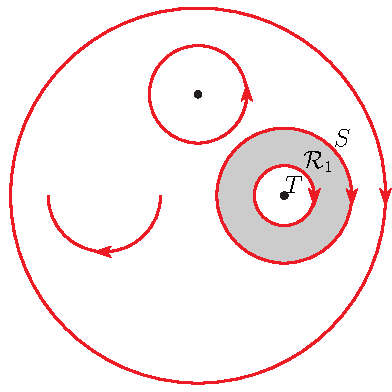
\includegraphics[scale=0.8]{OE10D_10i1.pdf}\qquad\qquad
       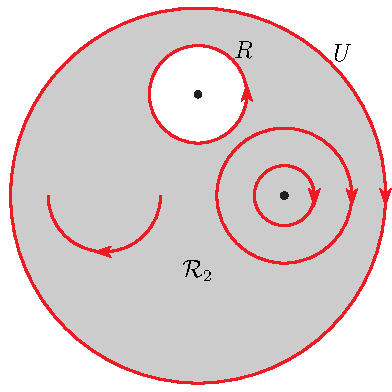
\includegraphics[scale=0.8]{OE10D_10i3.pdf}
  \end{center}

\item[(2)] False. Choose a coordinate system so that $Q$ is at the origin
and choose $\vF=\vG$.
We saw, in Examples \eref{CLP317}{eg:screeningCounterexample} and
\eref{CLP317}{eg:greenCC} of the CLP-4 text, that the curl of  
$\vG$ vanished everywhere except at the origin, where it was not defined,
but that $\int_R \vG\cdot\dee{\vr} \ne 0$.

\item[(3),(4)] False. Here is a counterxample that shows that both
(3) and (4) are false. Choose a coordinate system so that $Q$ is 
at the origin and choose $\vF=\vG$. By Stokes' theorem 
\begin{equation*}
\int_S \vG\cdot\dee{\vr} 
= \int_T \vG\cdot\dee{\vr} = 0
\end{equation*} 
because $\vnabla\times\vG=\vZero$ everywhere inside $S$, including at $P$.
So now both parts (3) and (4) reduce to the claim that 
$\int_U \vG\cdot\dee{\vr} 
= \int_R \vG\cdot\dee{\vr}$.

We saw, in Example \eref{CLP317}{eg:greenCC} of the CLP-4 text, that  $\int_R \vG\cdot\dee{\vr} = 2\pi$. 

To finish off the counterexample,
we'll now show that $\int_U \vG\cdot\dee{\vr} = -2\pi$.
Let $\cR_2$ be the region between $U$ and $R$. It is the shaded region 
in the figure on the right above. Note that $\vnabla\times\vG=\vZero$ 
on all of $\cR_2$. including at $P$.
The boundary of $\cR_2$ is $-U-R$, meaning that the boundary consists 
of two parts, with one part being $-U$ and the other part being $-R$. 
So, by Stokes' theorem
\begin{equation*}
-\int_U \vG\cdot\dee{\vr} - \int_R \vG\cdot\dee{\vr}
=\int_{\partial \cR_2} \vG\cdot\dee{\vr}
=\dblInt_{\cR_2} \vnabla\times\vG\cdot\hk\, \dee{S}
=0
\end{equation*}
and 
$\int_U \vG\cdot\dee{\vr} =-\int_R \vG\cdot\dee{\vr} = -2\pi$


\item[(5)] False. For any conservative vector field $\vF$, with potential $f$,
$\int_V \vF\cdot\dee{\vr}$ is just the difference of the values of $f$ at 
the two end points of $V$. It is easy to choose an $f$ for which those
two values are different. For example $f(x,y)=x$ does the job.


\end{itemize} 

\noindent (j)
Let $S$ be any closed surface and denote by $V$ the 
volume that it encloses. Presumably  the question assumes that
$S$ is oriented so that $S=\partial V$. Then by the divergence 
theorem
\begin{equation*}
\dblInt_S \vF \cdot \hn\,\dee{S}
=\dblInt_{\partial V} \vF \cdot \hn\,\dee{S}
=\tripInt_V \vnabla\cdot\vF\ \dee{V}
\end{equation*}
This is exactly the volume of $V$ if $\vnabla\cdot\vF=1$
everywhere. One vector field $\vF$ with $\vnabla\cdot\vF=1$
everywhere is $\vF=x\,\hi$.

\noindent (k)
Let $\cC$ be the counterclockwise boundary of a small square centred
on $P$, like the blue curve in the figure below, but much smaller. 
Call the square (the inside of $\cC$) $S$.

  \begin{center}
       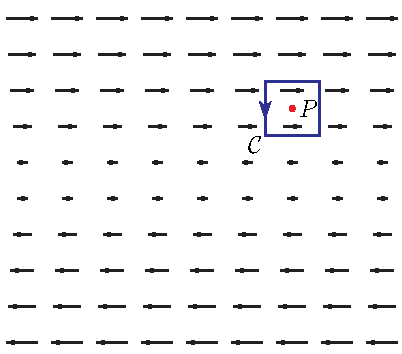
\includegraphics[scale=0.8]{shearFieldb.pdf}
  \end{center}

By Stokes' theorem
\begin{equation*}
\dblInt_S \vnabla\times\vF\cdot\hk\ \dee{S}
=\oint_\cC \vF\cdot\dee{\vr}
\end{equation*}
\begin{itemize}\itemsep1pt \parskip0pt \parsep0pt %\itemindent-15pt
\item[$\circ$]
The contribution to $\oint_\cC \vF\cdot\dee{\vr}$ coming from the left and
right sides of $\cC$ will be zero, because $\vF$ is perpendicular 
to $\dee{\vr}$ there. 
\item[$\circ$]
The contribution to $\oint_\cC \vF\cdot\dee{\vr}$ coming from the
top of $\cC$ will be negative, because there $\vF$ is a positive number times
$\hi$ and $\dee{\vr}$ is a negative number times $\hi$.
\item[$\circ$]
The contribution to $\oint_\cC \vF\cdot\dee{\vr}$ coming from the
bottom of $\cC$ will be positive, because there $\vF$ is a positive 
number times $\hi$ and $\dee{\vr}$ is a positive number times $\hi$.
\item[$\circ$]
The magnitude of the contribution from the top of $\cC$ will be
larger than the magnitude of the contribution from the bottom of $\cC$,
because $|\vF|$ is larger on the top than on the bottom.
\end{itemize} 
So, all together, $\oint_\cC \vF\cdot\dee{\vr}<0$, and consequently
(taking a limit as the square size tends to zero)
$\vnabla\times\vF\cdot\hk$ is negative at $P$.

\end{solution}

%%%%%%%%%%%%%%%%%%%%%%%%%%%
\begin{question}[M317 2010D] %10
Say whether the following statements are true or false.
\begin{enumerate}[(a)]
\item
If $\vF$ is a 3D vector field defined on all of $\bbbr^3$ , 
and $S_1$ and $S_2$ are two surfaces with the same boundary, but 
$\dblInt_{S_1} \vF\cdot\hn\,\dee{S} \ne  \dblInt_{S_2}  \vF\cdot\hn\,\dee{S}$, then $\vnabla\cdot\vF$ is not zero anywhere.

\item
If $\vF$ is a vector field satisfying $\vnabla\times\vF$ = 0 
whose domain is not simply-connected, then $\vF$ is not 
conservative.

\item
The osculating circle of a curve $C$ at a point has the same 
unit tangent vector, unit normal vector, and curvature as $C$ 
at that point.

\item
A planet orbiting a sun has period proportional to the cube of the 
major axis of the orbit.

\item
For any 3D vector field $\vF$, $\vnabla\cdot(\vnabla\times\vF)$ = 0.

\item
A field whose divergence is zero everywhere in its domain has
closed surfaces $S$ in its domain.

\item
The gravitational force field is conservative.

\item
If $\vF$ is a field defined on all of $\bbbr^3$ such that
$\int_C \vF \cdot \dee{\vr} = 3$ for some curve $C$, then $\vnabla\times\vF$
is non-zero at some point.

\item
The normal component of acceleration for a curve of constant curvature 
is constant.

\item
The curve defined by
\begin{equation*}
\vr_1(t) = \cos(t^4)\,\hi + 3t^4\hj,\qquad
-\infty < t < \infty,
\end{equation*}
is the same as the curve defined by
\begin{equation*}
\vr_2(t) = \cos t\,\hi + 3t\,\hk,\qquad
-\infty < t < \infty
\end{equation*}

\end{enumerate}
\end{question}

\begin{hint} 
Read all of the statements very carefully. The details are critical.

(a) Note the word \emph{anywhere}.

(b) If you have not learned about simply connected domains,
skip this part. If you have, read the statement very carefully.

(d) If you have not learned about Kepler's three laws, skip this part.

(h) Read the statement very carefully. It does not specify that $C$ is closed.

(i) Review \S\eref{CLP317}{sec:CurveCompendium} of the CLP-4 text.

\end{hint}

\begin{answer} 
(a) false \qquad
(b) false \qquad
(c) true \qquad
(d) false

(e) true, assuming that the second derivatives of the vector field exist 
and are continuous.

(f) silly, but true\qquad
(g) true\qquad
(h) false\qquad
(i) false\qquad
(j) false
\end{answer}

\begin{solution} (a) False. We could have, for example,
$\vnabla\cdot\vF$ zero at one point and strictly positive elsewhere.
One example would be $\vF = x^3\,\hi+y^3\,\hj +z^3\,\hk$, with $S_1$ and
$S_2$ being the upward oriented top and bottom hemispheres, respectively, 
of the unit sphere $x^2+y^2+z^2=1$.

(b) False. The conditions that (1) $\vnabla\times\vF$ = 0 and (2) the domain of
$\vF$ is simply-connected, are sufficient, but not necessary, 
to imply that $\vF$ is conservative. For example the vector field
$\vF=\vZero$, with any domain at all, is conservative with potential $0$.
Another example (which does not depend on choosing a domain that is smaller
than the largest possible domain) is $\vF=\vnabla\frac{1}{x^2+y^2}$
with domain $\Set{(x,y,z)}{ (x,y)\ne  (0,0)}$. That is, the domain is
$\bbbr^3$ with the $z$-axis removed.

(c) That's true. Consider any point $\vr(t_0)$ on a parametrized curve 
$\vr(t)$. That's the blue point in the figure below.
\vadjust{
  \begin{center}
       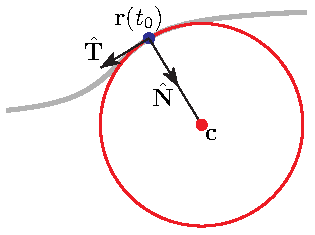
\includegraphics[scale=0.8]{circleCentreC.pdf}
  \end{center}
}The centre of curvature for the curve at $\vr(t_0)$ is
$\vc = \vr(t_0)+\rho(t_0)\hat\vN(t_0)$. It is the red dot in the figure.
\begin{itemize}\itemsep1pt \parskip0pt \parsep0pt %\itemindent-15pt
\item[$\circ$]
The radius of the osculating circle is the distance from its centre,
$\vc$, to any point of the circle,
like $\vr(t_0)$. That's $|\vr(t_0) -\vc| = |\rho(t_0)\hat\vN(t_0)| 
= \rho(t_0)$. 
The curvature of the osculating circle is one over its radius.
So its curvature is $\frac{1}{\rho(t_0)}=\ka(t_0)$.
\item[$\circ$]
The unit normal to the osculating circle at $\vr(t_0)$ is a unit
vector in the opposite direction to the radius vector from the centre
$\vc$ to $\vr(t_0)$. The radius vector is 
$\vr(t_0)-\vc_0=-\rho(t_0)\hat\vN(t_0)$, so the unit normal is $\hat\vN(t_0)$.
\item[$\circ$]
The osculating circle lies in the plane that best fits the curve
near $\vr(t_0)$. (See the beginning of \S\eref{CLP317}{sec:Curve3d}
in the CLP-4 text.) So the unit tangents to the osculating circle
at $\vr(t_0)$ are perpendicular to both $\hat\vN(t_0)$ and 
$\hat\vB(t_0)$ and so are either $\hat\vT(t_0)$ or $-\hat\vT(t_0)$,
depending on how we orient the osculating circle.
\end{itemize}

(d) False. Kepler's third law is that a planet orbiting a sun has 
the \emph{square} of the period proportional to the cube of the 
major axis of the orbit.

(e) True. That's part (a) of Theorem \eref{CLP317}{thm:degTwoIdentities}
in the CLP-4 text.

(f) True. Every domain contains closed surfaces. This has nothing to do
with vector fields.

(g) True. We saw this in Example \eref{CLP317}{eg:gravity} in the CLP-4 text.

(h) False. Let $\vF$ be an everywhere defined conservative vector field 
with potential $\varphi$. Then $\vnabla\times\vF=\vZero$ everywhere.
If $P$ and $Q$ are two points and if $\varphi(P)-\varphi(Q)=3$ and 
if $C$ is a curve from $Q$ to $P$, then $\int_C \vF \cdot \dee{\vr} = 3$. 
One example would be $\varphi(x,y,z) = x$, $\vF=\hi$, $P=(3,0,0)$, $Q=(0,0,0)$.

(i) False. The normal component of acceleration  depends on speed,
as well as curvature.

(j) False. The curve $\vr_1$ contains only points in the $xy$-plane. 
Every $\vr_2(t)$ with $t\ne 0$  has a nonzero $z$-coordinate.

\end{solution}

%%%%%%%%%%%%%%%%%%%%%%%%%%%
\begin{question}[M317 2009A] %9
Which of the following statements are true (T) and which are false (F)? 
% Write your answers in the following box. 
All real valued functions $f(x,y,z)$
and all vector fields $\vF(x, y, z)$ have domain $\bbbr^3$ unless 
specified otherwise.


%\begin{center}
%\begin{tabular}{ | c | c | c | c | c | c | c | c | c |}
%  \hline			
%      & 1 & 2 & 3 & 4 & 5 & 6 & 7 & 8 \\
%  \hline
%  T/F & \phantom{N}  & \phantom{N} & \phantom{N} & \phantom{N} & \phantom{N}
%      & \phantom{N}  & \phantom{N}  & \phantom{N} \\
%  \hline  
%\end{tabular}
%\end{center}


\begin{enumerate}[(a)]
\item
If $f$ is a continuous real valued function and $S$ a smooth oriented 
surface, then
\begin{equation*}
\dblInt_S f\, \dee{S} = -\dblInt_{-S} f\,\dee{S}
\end{equation*}
where `$-S$' denotes the surface $S$ but with the opposite orientation.

\item
Suppose the components of the vector field $\vF$ have continuous 
partial derivatives. If $\dblInt_S\vnabla\times\vF\cdot\hn\,\dee{S}=0$
for every closed smooth surface, then $\vF$ is conservative.

\item
Suppose $S$ is a smooth surface bounded by a smooth simple closed curve $C$. 
The orientation of $C$ is determined by that of $S$ as in Stokes' theorem. 
Suppose the real valued function $f$ has continuous partial derivatives. Then
\begin{equation*}
\int_C f\,\dee{x}
=\dblInt_S \left(\frac{\partial f}{\partial z}\hj
          - \frac{\partial f}{\partial y}\hk\right)\cdot\hn\,\dee{S}
\end{equation*}

\item
Suppose the real valued function $f(x,y,z)$ has continuous second order 
partial derivatives. Then
\begin{equation*}
(\vnabla f ) \times (\vnabla f ) = \vnabla  \times (\vnabla f )
\end{equation*}

\item
The curve parameterized by
\begin{equation*}
\vr(t) = \big(2 + 4t^3 \,,\, -t^3 \,,\, 1 - 2t^3\big)\qquad
-\infty < t < \infty
\end{equation*}
has curvature $\kappa(t) = 0$ for all $t$.

\item
If a smooth curve is parameterized by $\vr(s)$ where $s$ is arc length, 
then its tangent vector satisfies
\begin{equation*}
|\vr'(s)| = 1
\end{equation*}

\item
If $S$ is the sphere $x^2 + y^2 + z^2 = 1$ and $\vF$ is a constant 
vector field, then $\dblInt_S \vF \cdot\hn\, \dee{S} = 0$.

\item
There exists a vector field $\vF$ whose components have continuous second 
order partial derivatives such that $\vnabla\times\vF = (x, y, z)$.

\end{enumerate}
\end{question}

%\begin{hint} 
%
%\end{hint}

\begin{answer} 
(a) False\qquad
(b) False\qquad
(c) True\qquad
(d) True\qquad
(e) True\qquad
(f) True\qquad
(g) True\qquad
(h) False
\end{answer}

\begin{solution}
(a) False. Changing the orientation of a surface does not change $\dee{S}$
at all. (It changes $\hn\dee{S}$ by a factor of $(-1)$.) So 
\begin{equation*}
\dblInt_S f\, \dee{S} = +\dblInt_{-S} f\,\dee{S}
\end{equation*}
which is not $-\dblInt_{-S} f\,\dee{S}$, unless the integral is zero.

\noindent (b) False. For every vector field with two continuous
partial derivatives, $\vnabla\cdot(\vnabla\times\vF)=0$  (see Theorem
\eref{CLP317}{thm:degTwoIdentities}.a in the CLP-4 text), so 
the divergence theorem gives
\begin{align*}
\dblInt_S (\vnabla\times\vF) \cdot \hn\,\dee{S}
&=\tripInt_V \vnabla\cdot(\vnabla\times\vF)\,\dee{V}
=0
\end{align*}
whether or not $\vF$ is conservative.

\noindent (c) True. Define the vector field $\vF=f\,\hi$.
Then, by Stokes' theorem,
\begin{align*}
\int_C f\,\dee{x}
=\int_C \vF\cdot\dee{\vr}
=\dblInt_S\vnabla\times\vF\cdot\hn\,\dee{S}
=\dblInt_S \left(\frac{\partial f}{\partial z}\hj
          - \frac{\partial f}{\partial y}\hk\right)\cdot\hn\,\dee{S}
\end{align*}


\noindent (d) True.
The left hand side, $(\vnabla f ) \times (\vnabla f )$, is zero
because $(\vnabla f )$ is parallel to itself and the right hand side
$\vnabla  \times (\vnabla f )$ is zero by 
Theorem \eref{CLP317}{thm:degTwoIdentities}.b (the screening test for
conservative fields) of the CLP-4 text.


\noindent (e) True. The curve
$\vr(t) = \big(2 \,,\, 0\,,\, 1\big) +t^3\big(4 \,,\, -1 \,,\, -2\big)$ 
is a straight line. Straight lines have curvature $0$.

\noindent (f) True. In general $|\vr'(t)|=\diff{s}{t}$. Under arc
length parametrization $t=s$ so that $\diff{s}{t}=1$.

\noindent (g) True. If $\vF$ is a constant vector fleld, then, by the 
divergence thoerem,
\begin{equation*}
\dblInt_S \vF \cdot \hn\,\dee{S}
=\tripInt_V \vnabla\cdot\vF\,\dee{V}
=\tripInt_V 0\,\dee{V}
=0
\end{equation*}

\noindent (h) False. The statement $\vnabla\times\vF=(x,y,z)$ means
that $\vF$ is a vector potential for the vector field $\vG=(x,y,z)$.
But $\vG$ fails the screening test $\vnabla\cdot\vG=0$ for vector potentials.

\end{solution}

%%%%%%%%%%%%%%%%%%%%%%%%%%%
\begin{question}[M317 2008A] %3
The vector field
$\vF = P (x, y)\,\hi + Q(x, y)\,\hj$
is plotted below. 

\begin{center}
       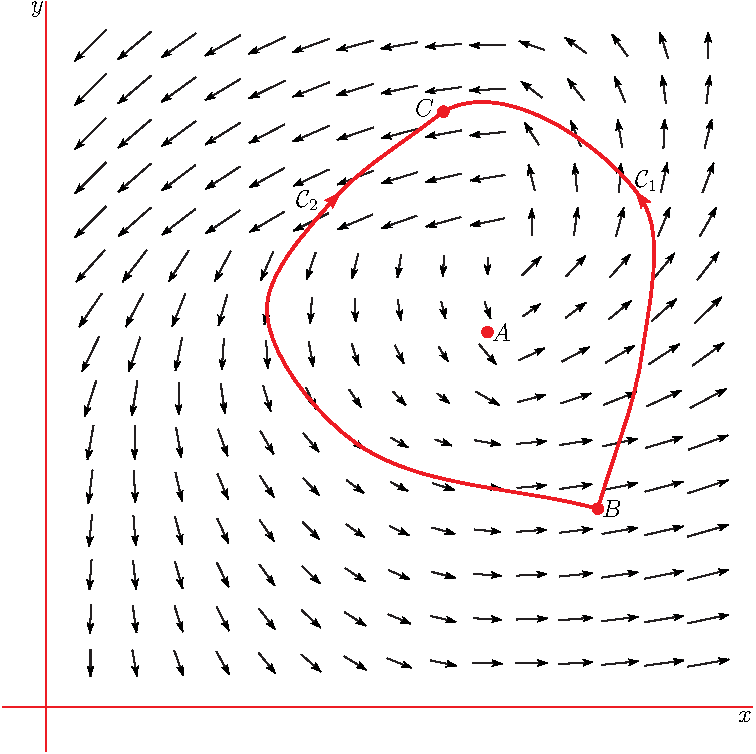
\includegraphics{OE08A_3.pdf}
\end{center}


In the following questions, give the answer that 
is best supported by the plot.
\begin{enumerate}[(a)]
\item
The derivative $P_y$ at the point labelled $A$ is 
   (a) positive, (b) negative, (c) zero, 
   (d) there is not enough information to tell.
\item
The derivative $Q_x$ at the point labelled $A$ is 
    (a) positive, (b) negative, (c) zero, 
    (d) there is not enough information to tell.
%\item
%The derivative $Q_x$ at the point labelled $A$ is 
%    (a) positive, (b) negative, (c) zero, 
%    (d) there is not enough information to tell.
%\item
%The derivative $Q_y$ at the point labelled $A$ is 
%    (a) positive, (b) negative, (c) zero, 
%    (d) there is not enough information to tell.
\item
The curl of $\vF$ at the point labelled $A$ is 
     (a) in the direction of $+\hk$ 
     (b) in the direction of $-\hk$ 
     (c) zero (d) there is not enough information to tell.
\item
The work done by the vector field on a particle travelling from point 
$B$ to point $C$ along the curve $\cC_1$ is 
    (a) positive (b) negative (c) zero 
    (d) there is not enough information to tell.
\item
The work done by the vector field on a particle travelling from point 
$B$ to point $C$ along the curve $\cC_2$ is 
    (a) positive (b) negative (c) zero 
    (d) there is not enough information to tell.
\item
The vector field $\vF$ is 
    (a) the gradient of some function $f$ 
    (b) the curl of some vector field $\vG$ 
    (c) not conservative 
    (d) divergence free.
\end{enumerate}
\end{question}

%\begin{hint} 
%

%\end{hint}

\begin{answer} 
(a) $P_y<0$ \qquad
(b) $Q_x>0$ \qquad
(c) $\vnabla\times\vF$ is in the direction of $+\hk$ at $A$

(d) $\int_{\cC_1}\vF\cdot\dee{\vr}>0$\qquad
(e) $\int_{\cC_2}\vF\cdot\dee{\vr}<0$\qquad
(f) $\vF$ is not conservative
\end{answer}

\begin{solution} 
(a) $P$ is the $x$-component of $\vF$. As we travel vertically upward 
through $A$, that $x$-component decreases. Hence $P_y<0$ at $A$.
 
(b) $Q$ is the $y$-component of $\vF$. As we travel horizontally to the
right through $A$, that $y$-component increases. Hence $Q_x>0$ at $A$.

(c) $\vnabla\times\vF = (Q_x-P_y)\hk$ and $Q_x-P_y>0$ at $A$, so that 
the curl of $\vF$ at $A$ is in the direction of $+\hk$. 

(d) Along the curve $\cC_1$ the magnitude of the angle between $\vF$ 
and $\dee{\vr}$ is less than $90^\circ$, so that $\vF\cdot\dee{\vr}>0$
and $\int_{\cC_1}\vF\cdot\dee{\vr}>0$.

(e) Along the curve $\cC_2$ the magnitude of the angle between $\vF$ 
and $\dee{\vr}$ is greater than $90^\circ$, so that $\vF\cdot\dee{\vr}<0$
and $\int_{\cC_2}\vF\cdot\dee{\vr}<0$.

(f) If $\vF$ were conservative, we would have $\int_{\cC_1}\vF\cdot\dee{\vr}
=\int_{\cC_2}\vF\cdot\dee{\vr}$. As these two integrals have opposite signs
$\vF$ is not conservative. (Since $\vF$ is not conservative, it is not the gradient of some function. At $A$, $P_x>0$ and $Q_y>0$. So $\vF$ is not divergence free and is not the curl of a vector potential.)


\end{solution}

%%%%%%%%%%%%%%%%%%%%%%%%%%%
\begin{question}[M317 2008A] %10
Which of the following statements are true (T) and which are false (F)?
%Write your answers in the following box. 
%
%\begin{center}
%\begin{tabular}{ | c | c | c | c | c | c | c | c | c | c | c |}
%  \hline			
%      & 1 & 2 & 3 & 4 & 5 & 6 & 7 & 8 &9 &10 \\
%  \hline
%  T/F & \phantom{N}  & \phantom{N} & \phantom{N} & \phantom{N} & \phantom{N}
%      & \phantom{N}  & \phantom{N}  & \phantom{N} & \phantom{N} & \phantom{N} \\
%  \hline  
%\end{tabular}
%\end{center}
\begin{enumerate}[(a)]
\item
The curve defined by
\begin{equation*}
\vr_1(t) = \cos(t^2 )\,\hi + \sin(t^2 )\,\hj + 2t^2\,\hk,\qquad
-\infty < t < \infty
\end{equation*}
is the same as the curve defined by
\begin{equation*}
\vr_2 (t) = \cos t\,\hi + \sin t\,\hj + 2t\,\hk,\qquad
-\infty < t < \infty
\end{equation*}

\item
The curve defined by
\begin{equation*}
\vr_1(t) = \cos(t^2)\,\hi + \sin(t^2 )\,\hj + 2t^2\,\hk,\qquad
0 \le t \le 1
\end{equation*}
is the same as the curve defined by
\begin{equation*}
\vr_2(t) = \cos t\,\hi + \sin t\,\hj + 2t\,\hk,\qquad
0 \le t \le 1
\end{equation*}


\item
If a smooth curve is parameterized by $\vr(s)$ where $s$ is arc length, 
then its tangent vector satisfies
\begin{equation*}
|\vr'(s)| = 1
\end{equation*}

\item
If $\vr(t)$ defines a smooth curve $C$ in space that has constant 
curvature $\kappa > 0$, then $C$ is part of a circle with radius $1/\kappa$.

\item
If the speed of a moving object is constant, then its acceleration 
is orthogonal to its velocity.

\item
The vector field
\begin{equation*}
\vF(x, y, z) = \frac{-y}{x^2+y^2} \hi 
               + \frac{x}{x^2+y^2} \hj
               + z\hk
\end{equation*}
is conservative.

\item
Suppose the vector field $\vF(x, y, z)$ is defined on an open domain 
and its components have continuous partial derivatives. If 
$\vnabla\times\vF = 0$, then $\vF$ is conservative.

\item
The region $D = \Set{ (x, y) }{ x^2 + y^2 > 1 }$ is simply connected.

\item
The region $D = \Set{ (x, y) }{ y - x^2 > 0 }$ is simply connected.

\item
If $\vF$ is a vector field whose components have two continuous 
partial derivatives, then
\begin{equation*}
\dblInt_S \vnabla\times \vF \cdot\hn\, \dee{S} = 0
\end{equation*}
when $S$ is the boundary of a solid region $E$ in $\bbbr^3$.

\end{enumerate}
\end{question}

\begin{hint} 
Read all of the statements very carefully. The details are critical.

For part (d), note that the curve need not lie in a plane.

For part (g), note that the domain can have holes in it.

For parts (h) and (i), by definition, $D$ is simply connected if 
any simply closed curve in $D$ can be shrunk to a 
point continuously in $D$.

\end{hint}

\begin{answer} 
(a) False\qquad
(b) True\qquad
(c) True\qquad
(d) False\qquad
(e) True\qquad
(f) False\qquad
(g) False\qquad
(h) False\qquad
(i) True\qquad
(j) True
\end{answer}

\begin{solution} 
(a) 
False. The curve $\vr_1$ contains only points with $z\ge0$. 
Every $\vr_2(t)$ with $t< 0$  has $z<0$.

(b) True. $\vr_2(t^2)=\vr_1(t)$ and $t^2$ runs from $0$ to $1$ as
$t$ runs from $0$ to $1$.

(c) True. In general $|\vr'(t)| = \diff{s}{t}$. When $t=s$, $\diff{s}{t}=1$.

(d) False. The curve need not even lie in a plane. For example, as we
saw in Example \eref{CLP317}{eg:helixTwist}  of the CLP-4 text, the helix
$\vr(t) = a\cos t\,\hi +b\sin t\,\hj + bt\,\hk$ has constant curvature
$\ka=\frac{a}{a^2+b^2}$ but is not a circle.

(e) True. If the speed $|\vv|=\sqrt{\vv\cdot\vv}$ of a moving object is constant, then
\begin{equation*}
0=\diff{\hfill}{t}\big(\vv\cdot\vv\big)=2\vv\cdot\va
\end{equation*}

(f) False. If the vector field
$
\vF(x, y, z) = \frac{-y}{x^2+y^2} \hi 
               + \frac{x}{x^2+y^2} \hj
               + z\hk
$
were conservative, its restriction, $\frac{-y}{x^2+y^2} \hi+ \frac{x}{x^2+y^2} \hj$,
to the $xy$-plane would also be conservative. But we saw in
Examples  \eref{CLP317}{eg:screeningCounterexample} and
\eref{CLP317}{eg:greenCC} of the CLP-4 text that the vector 
field $\frac{-y}{x^2+y^2} \hi+ \frac{x}{x^2+y^2} \hj$ is not conservative.  

(g) False. The vector field of part (f), with domain
$\Set{(x,y,z)}{ x^2+y^2>1}$, provides a counterexample.  

(h) False. The curve $x^2+y^2 = 2$ can not be shrunk to a 
point continuously in $\Set{ (x, y) }{ x^2 + y^2 > 1 }$.

(i) True. Any curve in $\Set{ (x, y) }{ y > x^2  }$ can be shrunk to a 
point continuously in $\Set{ (x, y) }{ y > x^2  }$.

(j) True. By the divergence theorem,
\begin{align*}
\dblInt_S \vnabla\times \vF \cdot\hn\, \dee{S}
=\tripInt_E \vnabla\cdot(\vnabla\times \vF)\, \dee{V}
=0
\end{align*}
since $\vnabla\cdot(\vnabla\times \vF)=0$ by the vector identity
of Theorem \eref{CLP317}{thm:degTwoIdentities}.a in the CLP-4 text.

\end{solution}


%%%%%%%%%%%%%%%%%%%%%%%%%%%
\begin{question}[M317 2007A] %10
Which of the following statements are true (T) and which are false (F)?
\begin{enumerate}[(a)]
\item
If a smooth curve $C$ is parameterized by $\vr(s)$ where $s$ 
is arc length, then the tangent vector $\vr'(s)$ satisfies 
$|\vr'(s)| = 1$.
\item
If $\vr(t)$ defines a smooth curve $C$ in space that has constant 
curvature $\kappa > 0$, then $C$ is part of a circle with radius $1/\kappa$.
\item
Suppose $\vF$ is a continuous vector field with open domain $D$. If
\begin{equation*}
\int_C \vF \cdot \dee{\vr} = 0
\end{equation*}
for every piecewise smooth closed curve $C$ in $D$, then $\vF$ is conservative.
\item
Suppose $\vF$ is a vector field with open domain $D$, and the components 
of $\vF$ have continuous partial derivatives. If $\vnabla\times \vF= 0$ everywhere on $D$, then $\vF$ is conservative.
\item
The curve defined by
\begin{equation*}
\vr_1(t) = \cos(t^2)\,\hi + \sin(t^2)\,\hj + 2t^2\,\hk,\qquad
-\infty < t < \infty
\end{equation*}
is the same as the curve defined by
\begin{equation*}
\vr_2 (t) = \cos t\,\hi + \sin t\,\hj + 2t\,\hk,\qquad
-\infty < t < \infty
\end{equation*}
\item
The curve defined by
\begin{equation*}
\vr_1(t) = \cos(t^2)\,\hi + \sin(t^2)\,\hj + 2t^2\,\hk,\qquad
0\le t \le 1
\end{equation*}
is the same as the curve defined by
\begin{equation*}
\vr_2 (t) = \cos t\,\hi + \sin t\,\hj + 2t\,\hk,\qquad
0\le t\le 1
\end{equation*}
\item
Suppose $\vF(x, y, z)$ is a vector field whose components have 
continuous second order partial derivatives. Then 
$\vnabla \cdot (\vnabla  \times F) = 0$.
\item
Suppose the real valued function $f(x, y, z)$ has continuous second 
order partial derivatives. Then $\vnabla\cdot(\vnabla f) = 0$.
\item
The region $D = \Set{ (x, y) }{ x^2 + y^2 > 1 }$ is simply connected.
\item
The region $D = \Set{ (x, y) }{ y - x^2 > 0 }$ is simply connected.


\end{enumerate}
\end{question}

\begin{hint} 
Read all of the statements very carefully. The details are critical.

For part (b), note that the curve need not lie in a plane.

For part (d), note that the domain can have holes in it.

For parts (i) and (j), by definition, $D$ is simply connected if 
any simply closed curve in $D$ can be shrunk to a 
point continuously in $D$.


\end{hint}

\begin{answer} 
(a) True\qquad
(b) False\qquad
(c) True\qquad
(d) False\qquad
(e) False\qquad
(f) True\qquad
(g) True\qquad
(h) False\qquad
(i) False\qquad
(j) True
\end{answer}

\begin{solution} 

(a) True. In general $|\vr'(t)| = \diff{s}{t}$. When $t=s$, $\diff{s}{t}=1$.

(b) False. The curve need not even lie in a plane. For example, as we
saw in Example \eref{CLP317}{eg:helixTwist} of the CLP-4 text, 
the helix $\vr(t) = a\cos t\,\hi +b\sin t\,\hj + bt\,\hk$ has constant 
curvature $\ka=\frac{a}{a^2+b^2}$ but is not a circle.

(c) True. See Theorem \eref{CLP317}{thm:pathIndepConserv} of the CLP-4 text.

(d) False. The vector field 
$
\vF(x, y, z) = \frac{-y}{x^2+y^2} \hi 
               + \frac{x}{x^2+y^2} \hj
$,
with domain 
\begin{equation*}
\Set{(x,y,z)}{ x^2+y^2>1}
\end{equation*} 
provides a counterexample.  

(e)  False. The curve $\vr_1$ contains only points with $z\ge0$. 
Every $\vr_2(t)$ with $t< 0$  has $z<0$.

(f) True. $\vr_2(t^2)=\vr_1(t)$ and $t^2$ runs from $0$ to $1$ as
$t$ runs from $0$ to $1$.

(g) True. $\vnabla\cdot(\vnabla\times \vF)=0$ by the vector identity
of Theorem \eref{CLP317}{thm:degTwoIdentities}.a in the CLP-4 text.

(h) False. A counterexample is $f(x,y,z) = x^2$. It has
     $\vnabla f = 2 x\,\hi$ and hence $\vnabla\cdot(\vnabla f) = 2$.


(i) False. The curve $x^2+y^2 = 2$ can not be shrunk to a 
point continuously in $\Set{ (x, y) }{ x^2 + y^2 > 1 }$.

(j) True. Any curve in $\Set{ (x, y) }{ y > x^2  }$ can be shrunk to a 
point continuously in $\Set{ (x, y) }{ y > x^2  }$.

\end{solution}

%%%%%%%%%%%%%%%%%%%%%%%%%%%
\begin{question}[M317 2006A] %1
Let $\vF$, $\vG$ be vector fields, and $f$, $g$ be scalar fields.
Assume $\vF$, $\vG$, $f$, $g$ are defined on all of $\bbbr^3$ and
have continuous partial derivatives of all orders everywhere.
Mark each of the following as True (T) or False (F).

\begin{enumerate}[(a)]
\item
If $C$ is a closed curve and $\vnabla f=\vZero$, then $\int_C f\,\dee{s}=0$.
\item
If $\vr(t)$ is a parametrization of a smooth curve $C$ and the binormal
$\vB(t)$  is constant then $C$ is a straight line.
\item
If $\vr(t)$ is the position of a particle which travels with constant speed,
then $\vr'(t)\cdot\vr''(t)=0$. 
\item
If $C$ is a path from points $A$ to $B$, then the line integral $\int_C\big(\vF\times\vG\big)\cdot\dee{\vr}$ is independent of 
the path $C$.
\item
The line integral $\int_C f\,\dee{s}$ does not depend of the orientation of
the curve $C$.
\item
If $S$ is a parametric surface $\vr(u,v)$ then a normal to $S$ is given
by
\begin{align*}
\frac{\partial\vr}{\partial u}\times \frac{\partial\vr}{\partial u}
\end{align*}
\item
The surface area of the parametric surface $S$ given by 
$\vr(u,v) = x(u,v)\,\hi + y(u,v)\,\hj + z(u,v)\,\hk$, $(u,v)\in D$, is
given by
\begin{align*}
\dblInt_D \left(1+\big(\tfrac{\partial z}{\partial u}\big)^2
             +\big(\tfrac{\partial z}{\partial v}\big)^2\right)^{1/2}                  \dee{u}\dee{v}
\end{align*}
\item
If $\vF$ is the velocity field of an incompressible fluid then 
$\vnabla\cdot\vF=0$.
\item
$\vnabla\cdot\big(\vF\times\vG\big) 
= (\vnabla\cdot\vF)\vG + (\vnabla\cdot\vG)\vF$
\end{enumerate}
\end{question}

\begin{hint} 
Read all of the statements very carefully. The details are critical.

(a) The integral $\int_C f\,\dee{s}=0$ is not of the form 
     $\int_C \vF \cdot \dee{\vr}$.

(d) $\vF$ and $\vG$ can be any vector fields.

(e) Think about how $\int_C f\,\dee{s}$ is defined.

(f) Look at $\frac{\partial\vr}{\partial u}\times 
          \frac{\partial\vr}{\partial u}$ \emph{very} closely.

(g) The integral is completely independent of $x(u,v)$ and $y(u,v)$.

\end{hint}

\begin{answer} 
(a) False.\qquad
(b) False.\qquad
(c) True.\qquad
(d) False.\qquad
(e) True.\qquad
(f) False.

(g) False.\qquad
(h) True.\qquad
(i) False.

\end{answer}

\begin{solution}
(a) False. $\vnabla f=\vZero$ if and only if $f$ is constant. But
if $f$ is the constant $K$, then $\int_C f\,\dee{s}$ is $K$ times the
length of $C$, which need not be zero.

(b) False. Any curve which lies in a plane has constant binormal.
For example, the circle $\vr(t) =\cos t\,\hi +\sin t\,\hj +0\,\hk$ 
has constant binormal $\hat\vB=\hk$, but is not a straight line.

(c) True. If $\vr(t)$ has constant speed, the $\big(\diff{s}{t}(t)\big)^2
=\vr'(t)\cdot\vr'(t)$ is constant and
\begin{align*}
0= \diff{\hfill}{t} \big(\vr'(t)\cdot\vr'(t)\big)
= 2\vr'(t)\cdot\vr''(t)
\end{align*}

(d) False. For the line integral $\int_C\big(\vF\times\vG\big)\cdot\dee{\vr}$ 
to be independent of the path $C$, the vector field $\vF\times\vG$
has to be conservative and so has to obey $\vnabla\times(\vF\times\vG)=\vZero$.
But
\begin{itemize}\itemsep1pt \parskip0pt \parsep0pt %\itemindent-15pt
\item[$\circ$]
Not all vector fields are conservative. For example, the vector field
$\vH = x\,\hj$ obeys $\vnabla\times\vH = \hk$ and so is not conservative.
\item[$\circ$]
We can make $\vF\times\vG$ be \emph{any} vector field through judicious
choices of $\vF$ and $\vG$. For example, if $\vF= x\,\hk$ and $\vG = \hi$, 
then $\vF\times\vG=x\,\hk\times\hi=x\,\hj=\vH$.
\end{itemize}


(e) True. The contribution to $\int_C f\,\dee{s}$ from an
``infinitesmal piece of $C$'' is the value of $f$ on the piece
times the \emph{length} of the piece. That does not depend on the
orientation of the piece.

(f) False. The two vectors in the cross product 
$\frac{\partial\vr}{\partial u}\times \frac{\partial\vr}{\partial u}$
are identical. So the cross product is $\vZero$.

(g) False. The integral is completely independent of $x(u,v)$ and $y(u,v)$.
In particular if, for example, $x(u,v)= 157u$, $y(u,v)=157v$, $z(u,v)=0$ then
$\dblInt_D \left(1+\big(\tfrac{\partial z}{\partial u}\big)^2
             +\big(\tfrac{\partial z}{\partial v}\big)^2\right)^{1/2}                  \dee{u}\dee{v}$
is always exactly the area of $D$, while the area of $S$ is $157^2$ times the
area of $D$.

(h) True. If the fluid is incompressible then its flow preserves volumes
and consequently $\vnabla\cdot\vF=0$.

(i) Not only False, but Ridiculous. The left had side is  scalar valued
while the right hand side is vector valued.

\end{solution}

%%%%%%%%%%%%%%%%%%%%%%%%%%%
\begin{question}[M317 2005D] %2
Say whether the following statements are true (T) or false
(F). You may assume that all functions and vector fields are defined 
everywhere and have derivatives of all orders everywhere.


\begin{enumerate}[(a)]
\item
The divergence of $\vnabla\times\vF$ is zero, for every $\vF$.
\item
In a simply connected region, $\int_C \vF\cdot\dee{\vr}$ 
depends only on the endpoints of $C$.
\item
If $\vnabla f = 0$, then $f$ is a constant function.
\item
If $\vnabla\times\vF = \vZero$, then $\vF$ is a constant vector field.
\item
If $\vnabla\cdot\vF = 0$, then $\dblInt_S\vF\cdot\hn\, \dee{S} = 0$ 
for every closed surface $S$.
\item
If $\int_C \vF\cdot \dee{\vr} = 0$ for every closed curve $C$, then 
$\vnabla \times\vF = 0$.
\item
If $\vr(t)$ is a path in three space with constant speed $|\vv(t)|$, 
then the acceleration is perpendicular to the tangent vector, i.e. 
$\va\cdot\hat\vT = 0$.
\item
If $\vr(t)$ is a path in three space with constant curvature $\kappa$, 
then $\vr(t)$ parameterizes part of a circle of radius $1/\kappa$.
\item
Let $\vF$ be a vector field and suppose that $S_1$ and $S_2$ 
are oriented surfaces with the same boundary curve $C$, and $C$ 
is given the direction that is compatible with the orientations
of $S_1$ and $S_2$ . Then $\dblInt_{S 1} \vF\cdot\hn\, \dee{S} 
= \dblInt_{S 2} \vF\cdot\hn\, \dee{S}$.
\item
Let $A(t)$ be the area swept out by the trajectory of a planet from time 
$t=0$ to time $t$. The $\diff{A}{t}$ is constant.
\end{enumerate}

\end{question}

\begin{hint} 
Read all of the statements very carefully. The details are critical.

(b) Read the statement very carefully.
  ``simply connected'' plays no role here. 
    The vector field $\vF$ is not required to be conservative.

(e) Recall that $S$ is closed when it is the boundary of a solid region $V$.

(g) Assume that the constant $|\vv|$ is not zero. 


(j) If you have not learned about Kepler's three laws, skip this part.



\end{hint}

\begin{answer} 
(a) True\qquad
(b) False\qquad
(c) True\qquad
(d) False\qquad
(e) True\qquad
(f) True\qquad
(g) True\qquad
(h) False\qquad
(i) False\qquad
(j) True

\end{answer}

\begin{solution}
(a) True. That $\vnabla\cdot(\vnabla\times\vF)=0$ is the vector identity of
    Theorem \eref{CLP317}{thm:degTwoIdentities}.a. That
    identity is the basis of the vector potential screening test.

(b) False. If $\vF$ is not conservative, then $\int_C \vF\cdot\dee{\vr}$
    will depend on the endpoints of $C$.

(c) True. If $\vnabla f = 0$, then
\begin{align*}
\frac{\partial f}{\partial x}(x,y,z)&=0 &&\implies &
         f(x,y,z)&=g(y,z) \\
\frac{\partial f}{\partial y}(x,y,z)&=0 &&\implies &
                 \frac{\partial g}{\partial y}(y,z)&=0 &&\implies &
         g(y,z)&=h(z) \\
\frac{\partial f}{\partial z}(x,y,z)&=0 &&\implies &
                 h'(z)&=0 &&\implies &
         h(z)&=C 
\end{align*}
for some functions $g(y,z)$, $h(z)$ and constant $C$.

(d) False. The curl $\vnabla\times\vF$ is zero for every conservative
vector fields $\vF$. There are many nonconstant conservative vector fields,
like $\vF(x,y,z) = x\,\hi$.

(e) True. As $S$ is closed, it is the boundary of a solid region $V$.
Then, by the divergence theorem,
\begin{equation*}
\dblInt_S\vF\cdot\hn\, \dee{S}
=\tripInt_V\vnabla\cdot\vF\,\dee{V}
=0
\end{equation*}

(f) True. If $\int_C \vF\cdot \dee{\vr} = 0$ for every closed curve $C$, 
then $\vF$ is conservative by Theorem  \eref{CLP317}{thm:pathIndepConserv}
in the CLP-4 text. 
Consequently, $\vnabla \times\vF = 0$ by Theorem \eref{CLP317}{thm:screen}.

(g) True. If the speed $|\vv|$ is constant then
\begin{align*}
0= \diff{\hfill}{t} |\vv|^2
= \diff{\hfill}{t} (\vv\cdot\vv)
= 2\vv\cdot\va
\end{align*}
Since $\hat\vT=\frac{\vv}{|\vv|}$, $\hat\vT\cdot\va=0$ too.
Here, we have assumed that the constant $|\vv|$ is not zero.
If the constant $|\vv|$ is zero, then $\hat\vT$ is not defined at all
(and $\va=0$). 

(h) False. The trap here is that the curve is in $\bbbr^3$, not $\bbbr^2$. 
As we saw in Example \eref{CLP317}{eg:helixTwist} of the CLP-4 text, 
a helix has constant curvature, but does not lie in a plane and so 
is not part of a circle. 

(i) False. The trap here is that we are told nothing about $\vnabla\cdot\vF$.
As an example, let $S_1$ be the hemisphere
\begin{equation*}
S_1=\Set{(x,y,z)}{x^2+y^2+z^2=1,\ z\ge 0}
\end{equation*}
with upward pointing normal and $S_2$ be the disk
\begin{equation*}
S_2=\Set{(x,y,0)}{x^2+y^2\le 1}
\end{equation*}
also with upward pointing normal.

\begin{center}
       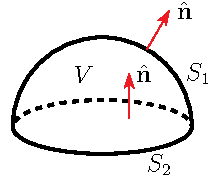
\includegraphics{OE05D_2i.pdf}
\end{center}

Set
\begin{equation*}
V=\Set{(x,y,z)}{0\le z\le \sqrt{x^2+y^2},\ x^2+y^2\le 1}
\end{equation*}
Then the boundary, $\partial V$, of $V$ consists of two parts, namely $S_1$
(with normal pointing upwards) and $S_2$ (but with normal pointing downwards).  The divergence theorem (Theorem \eref{CLP317}{thm:divThm} of the CLP-4 text) 
gives
\begin{align*}
\dblInt_{S_1} \vF \cdot \hn\,\dee{S}
-\dblInt_{S_2} \vF \cdot \hn\,\dee{S}
&=\tripInt_V \vnabla\cdot\vF\,\dee{V}
\end{align*}
If $\vnabla\cdot\vF>0$ (as is the case, for example, if $\vF=x\,\hi$)
then $\dblInt_{S_1} \vF \cdot \hn\,\dee{S}
-\dblInt_{S_2} \vF \cdot \hn\,\dee{S}$ is definitely nonzero.

(j) True. This is one of Kepler's laws. See \S\eref{CLP317}{sec:central forces}
in the CLP-4 text.


\end{solution}

%%%%%%%%%%%%%%%%%%%%%%%%%%%
\begin{question}[M317 2005D] %4
Find the correct identity, if $f$ is a function and $\vG$ and $\vF$ 
are vector fields. Select the true statement.
\begin{enumerate}[(a)]
\item\ \ 
$\vnabla\cdot(f \vF) = f \vnabla\times(\vF) + (\vnabla f ) \times\vF$
\item\ \ 
$\vnabla\cdot(f \vF) = f \vnabla\cdot(\vF) + \vF\cdot \vnabla f$
\item\ \ 
$\vnabla\times(f \vF) = f \vnabla\cdot(\vF) + \vF\cdot \vnabla f$
\item
None of the above are true.
\end{enumerate}
\end{question}

%\begin{hint} 
%
%\end{hint}

\begin{answer} 
(b)
\end{answer}

\begin{solution}
It's (b). 
(a) is gibberish --- the left hand side is a scalar while the right 
                      hand side is a vector.
(c) is also gibberish --- the left hand side is a vector while the right 
                      hand side is a scalar.
(b) is the vector identity of Theorem \eref{CLP317}{thm:divIdentities}.c
in the CLP-4 text.
\end{solution}


%%%%%%%%%%%%%%%%%%%%%%%%%%%
\begin{question}[M317 2005A] %8
True or False. Consider vector fields $\vF$ and scalar functions
$f$ and $g$ which are defined and smooth in all of three-dimensional space.
Let $\vr=(x,y,z)$ represent a variable point in space, and let 
$\vom = (\om_1,\om_2,\om_3)$ be a constant vector. Let $\Om$ be a smoothly 
bounded domain with outer normal $\hn$. Which of the following are identites, always valid under these assumptions?
\begin{enumerate}[(a)]
\item\ \ 
$\vnabla\cdot\vnabla f = 0$
\item\ \ 
$\vF\times\vnabla f = f\,\vnabla\cdot\vF$
\item\ \ 
$\vnabla^2 f = \vnabla(\vnabla\cdot f)$
\item\ \ 
$\vnabla\times\vnabla f = \vZero$
\item\ \ 
$(\vnabla\times f)+(\vnabla\times g)  = \vnabla f\times\vnabla g$
\item\ \ 
$\vnabla\cdot\vnabla\times\vF = 0$
\item\ \ 
$\vnabla\cdot\frac{\vr}{|\vr|^2} = 0$ for $\vr\ne\vZero$
\item\ \ 
$\vnabla\times(\vom\times\vr) = \vZero$
\item\ \ 
$\displaystyle\tripInt_\Om f\vnabla\cdot\vF\,\dee{V}
 =-\tripInt_\Om \vnabla f\cdot\vF\,\dee{V} 
 +\dblInt_{\partial\Om} f\vF\cdot\hn\,\dee{S}$
\item\ \ 
$\displaystyle\dblInt_{\partial\Om} f\hn\,\dee{S}
  =- \tripInt_\Om \vnabla f\,\dee{V}$
\end{enumerate}


\end{question}

\begin{hint} 
(g) Be careful. The power in the denominator is important.

(j) Beware the sign.
\end{hint}

\begin{answer} 
(a) False.\qquad
(b) False.\qquad
(c) False.\qquad
(d) True.\qquad
(e) False.\qquad
(f) True.\qquad
(g) False.\qquad
(h) False.\qquad
(i) True.\qquad
(j) False.
\end{answer}

\begin{solution}
(a) False. For example, if $f(x,y,z)=x^2$, then $\vnabla f = 2x\,\hi$
and $\vnabla\cdot\vnabla f = 2$.

(b) Not only false, but ridiculous. The left hand side is a vector while
the right hand side is a scalar.

(c) Not only false, but ridiculous. The right hand side is a vector while
the left hand side is a scalar.

(d) True. That's the screening test for conservative fields,
Theorem \eref{CLP317}{thm:degTwoIdentities}.b in the CLP-4 text.

(e) Not only false, but ridiculous. The curl of a scalar function
is not defined.

(f) True. That's the screening test for vector potentials,
Theorem \eref{CLP317}{thm:degTwoIdentities}.a in the CLP-4 text.

(g) False.
\begin{align*}
&\vnabla\cdot\frac{\vr}{|\vr|^2} 
=\frac{\partial\hfill}{\partial x}\frac{x}{x^2+y^2+z^2}
+\frac{\partial\hfill}{\partial y}\frac{y}{x^2+y^2+z^2} 
+\frac{\partial\hfill}{\partial z}\frac{z}{x^2+y^2+z^2}
\\
&\hskip0.25in
=\frac{1}{x^2+y^2+z^2} - \frac{2x^2}{{[x^2+y^2+z^2]}^2}
+\frac{1}{x^2+y^2+z^2} - \frac{2y^2}{{[x^2+y^2+z^2]}^2}
    \\&\hskip2in
+\frac{1}{x^2+y^2+z^2} - \frac{2z^2}{{[x^2+y^2+z^2]}^2}
\\
&\hskip0.25in
=\frac{3[x^2+y^2+z^2] - 2x^2-2y^2-2z^2}{{[x^2+y^2+z^2]}^2}
\\
&\hskip0.25in
=\frac{1}{x^2+y^2+z^2}
\end{align*}

(h) False.
For any constant vector $\vom=(\omega_1,\omega_2,\omega_3)$,
\begin{align*}
\vom\times\vr
&=\det\left[\begin{matrix}
\hi &\hj &\hk \\
\omega_1 & \omega_2 & \omega_3 \\
x   &  y  & z
\end{matrix}
\right]
= (\omega_2 z - \omega_3 y)\hi 
 -(\omega_1 z - \omega_3 x)\hj
 +(\omega_1 y - \omega_2 x)\hj
\end{align*}
So 
\begin{align*}
\vnabla\times(\vom\times\vr)
&=\det\left[\begin{matrix}
\hi &\hj &\hk \\
\tfrac{\partial\hfill}{\partial x} & \tfrac{\partial\hfill}{\partial y} & 
                \tfrac{\partial\hfill}{\partial z} \\
\omega_2 z - \omega_3 y & -\omega_1 z + \omega_3 x & \omega_1 y - \omega_2 x
\end{matrix}
\right]
=2 \omega_1\hi + 2 \omega_2\hj + 2 \omega_3\hk 
\end{align*}
is nonzero, unless the constant vector $\vom=\vZero$.

(i) True. The given equation is equivalent (by the vector identity Theorem \eref{CLP317}{thm:divIdentities}.c in
the CLP-4 text) to
\begin{equation*}
\tripInt_\Om \vnabla\cdot\big(f\vF\big)\,\dee{V}
 =\dblInt_{\partial\Om} f\vF\cdot\hn\,\dee{S}
\end{equation*}
which is true by the divergence theorem.

(j) False. One of the variants of the divergence theorem given
in Theorem \eref{CLP317}{thm:divVrn} of the CLP-4 text is
\begin{equation*}
\dblInt_{\partial\Om} f\hn\,\dee{S}
  = \tripInt_\Om \vnabla f\,\dee{V}
\end{equation*}
Note that the sign on the right hand side is ``$+$'', not ``$-$''.
In order for the equation given in part (j) to be true, it would
be necessary that $\tripInt_\Om \vnabla f\,\dee{V}=0$ for all smooth
scalar functions $f$. That's silly. One counterexample is 
\begin{equation*}
f(x) = x\qquad
\Omega = \Set{(x,y,z)}{x^2+y^2+z^2\le 1}
\end{equation*}
Then
\begin{align*}
\dblInt_{\partial\Om} f\hn\,\dee{S}
&=\dblInt_{\partial\Om}x(\overbrace{x\,\hi+y\,\hj+z\,\hk}^{\hn})\,\dee{S}
=\hi \dblInt_{\partial\Om}x^2\,\dee{S}
\\
- \tripInt_\Om \vnabla f\,\dee{V}
&=- \tripInt_\Om \hi\,\dee{V}
=- \hi\tripInt_\Om \dee{V}
\end{align*}
The coefficient of $\hi$ is obviously strictly positive in the upper
integral and  strictly negative in the lower integral. 

\end{solution}

%%%%%%%%%%%%%%%%%%%%%%%%%%%%%%%
\begin{question}[M317 2011A] %8
Determine if the given statements are True or False. Provide a reason or a counterexample.
\begin{enumerate}[(a)]
\item
A constant vector field is conservative on $\bbbr^3$.
\item
If $\vnabla\cdot\vF= 0$ for all points in the domain of $\vF$
then $\vF$ is a constant vector field.
\item
Let $\vr(t)$  be a parametrization of a curve $C$ in $\bbbr^3$.
If $\vr(t)$ and $\diff{\vr}{t}$ are orthogonal at all
points of the curve $C$, then $C$ lies on the surface of a sphere 
$x^2 + y^2 + z^2 = a^2$ for some $a>0$.
\item
The curvature $\kappa$ at a point on a curve depends on the orientation 
of the curve.
\item
The domain of a conservative vector field must be simply connected.

\end{enumerate}
\end{question}

%\begin{hint} 
%
%\end{hint}

\begin{answer} 
(a) True\qquad
(b) False\qquad
(c) True, assuming that $\vr(t)$ is not indentically $\vZero$.

(d) False\qquad
(e) False 
\end{answer}

\begin{solution} 
(a) True. If the vector field is $\vF = a\,\hi +b\,\hj + c\,\hk$,
then $f(x,y,z) = ax + by + cz$ obeys $\vF=\vnabla f$ and so
is a potential for $\vF$.

(b) False. For example the vector field $\vF= x\,\hi-y\,\hj$
obeys $\vnabla\cdot\vF= 0$ but is not a constant vector field.

(c) True, assuming that $\vr(t)$ is not indentically $\vZero$.
If $\vr(t)$ and $\diff{\vr}{t}$ are orthogonal at all
points of the curve $C$, then
\begin{equation*}
\diff{\hfill}{t} \big(\vr(t)\cdot\vr(t)\big)
  = 2\vr(t)\cdot\diff{\vr}{t}(t)
  =0
\end{equation*}
So $x(t)^2 + y(t)^2 + z(t)^2 = \vr(t)\cdot\vr(t)$ is a constant.
If $\vr(t)$ is not indentically $\vZero$, that constant must
be strictly positive. That is $x(t)^2 + y(t)^2 + z(t)^2 = a^2$
for some constant $a>0$.

(d) False. The curvature (see \S\eref{CLP317}{sec:CurveCompendium}
in the CLP-4 text) is
\begin{equation*}
\ka(t)= \frac{\Big|\diff{\hat\vT}{t}(t)\Big|}{|\vr'(t)|}
\end{equation*}
Changing the orientation of the curve amounts to replacing $t$ by $-t$.
This changes the signs of $\hat\vT$ and $\vr'$,
but does not change $\ka$, because the absolute values eliminate the signs.

(e) False. For example, the vector field $\vF=\vZero$, with domain
$\Set{(x,y,z)}{x^2+y^2>0}$ is a conservative vector field 
(with potential $0$) whose domain is not simply connected. As a less
nitpicky example, let $\vF=\vnabla f$ with $f=\frac{1}{x^2+y^2}$. The biggest
possible domain for this vector field is also $\Set{(x,y,z)}{x^2+y^2>0}$.
\end{solution}

%%%%%%%%%%%%%%%%%%%%%%%%%%%%%%%
\begin{question}[M317 2012J] %1
Provide a short answer to each question.
\begin{enumerate}[(a)]
\item
Compute $\vnabla\cdot\big(x^2 y\,\hi + e^y \sin x\,\hj + e^{zx}\,\hk\big)$
\item
Compute $\vnabla\times(\cos x^2\,\hi - y^3 z\,\hj + xz\,\hk\big)$
\item
Let
\begin{equation*}
\vF = \frac{x}{x^2+y^2}\hi +\frac{y}{x^2+y^2}\hj +z^2\,\hk
\end{equation*}
and let $D$ be the domain of $\vF$. Consider the following four
statments.
\begin{enumerate}[(I)]
\item  $D$ is connected
\item  $D$ is disconnected
\item  $D$ is simply connected
\item  $D$ is not simply connected
\end{enumerate}
Choose one of the following:
\begin{enumerate}[(i)]
\item (II) and (III) are true
\item (I) and (III) are true
\item (I) and (IV) are true
\item (II) and (IV) are true
\item Not enough information to determine
\end{enumerate}

\item
True or False? If the speed of a particle is constant then the 
acceleration of the particle is zero. If your answer is \textbf{True}, 
provide a reason. If your answer is \textbf{False}, provide a counter example.

\end{enumerate}
\end{question}

%\begin{hint} 
%
%\end{hint}

\begin{answer} 
\item %1
(a) $2xy + e^y\sin x + xe^{xz}$\qquad
(b) $y^3\,\hi-z\,\hj$\qquad
(c) (iii)\qquad
(d) False.
\end{answer}

\begin{solution} 
(a) We are to compute the divergence of 
$x^2 y\,\hi + e^y \sin x\,\hj + e^{zx}\,\hk$. Since
\begin{alignat*}{3}
\frac{\partial\hfill}{\partial x}\big(x^2 y\big)
&=2xy
\\
\frac{\partial\hfill}{\partial y}\big(e^y \sin x\big)
&= e^y\sin x
\\
\frac{\partial\hfill}{\partial z}\big(e^{zx}\big)
&=xe^{xz}
\end{alignat*}
the specified divergence is
\begin{align*}
\vnabla\cdot\big(x^2 y\,\hi + e^y \sin x\,\hj + e^{zx}\,\hk\big) 
        &= 2xy + e^y\sin x + xe^{xz}
\end{align*}

(b) The specified curl is
\begin{align*}
\vnabla\times\big(\cos x^2\,\hi - y^3 z\,\hj + xz\,\hk\big)
&=\det\left[\begin{matrix}\hi&\hj&\hk\\[0.03in] 
     \frac{\partial\hfill}{\partial x}&
        \frac{\partial\hfill}{\partial y}&
        \frac{\partial\hfill}{\partial z}\\[0.03in]
\cos x^2 & - y^3 z & xz\end{matrix}\right]
= y^3\,\hi-z\,\hj
\end{align*}

(c) In principle, the domain could be any subset of $\Set{(x,y,z)}{x^2+y^2>0}$.
We are not told which subset to use, so, by default, $D$ is the maximal
domain
\begin{equation*}
D=\Set{(x,y,z)}{x^2+y^2>0} = \Set{(x,y,z)}{(x,y)\ne (0,0)}
\end{equation*} 
This $D$ is connected (any two points in $D$
can be joined by a curve that lies completely in $D$) but is not
simply connected (the simple closed curve $\vr(\theta)=\cos\theta\,\hi
+\sin\theta\,\hj$, $0\le\theta\le 2\pi$ lies in $D$ but cannot be shrunk 
to a point continuously in $D$). So (I) and (IV) are true. That's (iii).

(d) False. If the position of the particle at time $t$ is
$\vr(t) = \cos t\,\hi +\sin t\,\hj$, then its speed is the constant $1$ 
but its acceleration is $-\cos t\,\hi -\sin t\,\hj$, which is nonzero.
\end{solution}


%%%%%%%%%%%%%%%%%%%%%%%%%%%%%%%
\begin{question}[M317 2016D] %10
Are each of the following statements True or False? 
Recall that $f \in C^k$ means that all derivatives of $f$ up to order 
$k$ exist and are continuous.

\begin{enumerate}[(a)]
\item
$\vnabla\times(f \vnabla f ) = \vZero$ for all $C^2$ scalar functions $f$ 
in $\bbbr^3$.

\item
$\vnabla\cdot(f\vF) = \vnabla f \cdot\vF + f\vnabla\cdot \vF $
for all $C^1$ scalar functions $f$ and $C^1$ vector fields $\vF$ in $\bbbr^3$.

\item
A smooth space curve $C$ with constant curvature $\kappa = 0$ must be a
part of a straight line.

\item
A smooth space curve $C$ with constant curvature $\kappa \ne 0$ must be 
part of a circle of radius $1/\kappa$.

\item
If $f$ is any smooth function defined in $\bbbr^3$ and if $C$ is any 
circle, then $\int_C\vnabla f\cdot\dee{\vr}=0$.


\item
Suppose $\vF$ is a smooth vector field in $\bbbr^3$ and $\vnabla\cdot\vF=0$
everywhere. Then, for every sphere, the flux \emph{out} of one hemisphere 
is equal to the flux \emph{into} the opposite hemisphere.

\item
Let $\vF(x, y,z)$ be a continuously differentiable vector field which is 
defined for every $(x, y, z)$. Then, 
$\dblInt_S\vnabla\times\vF\cdot\hn\,\dee{S}=0$ for any closed surface $S$.
(A closed surface is a surface that is the boundary of a solid region.)

\end{enumerate}
\end{question}

%\begin{hint} 
%
%\end{hint}

\begin{answer} 
(a) True\qquad
(b) True\qquad
(c) True\qquad
(d) False\qquad
(e) True\qquad
(f) True\qquad
(g) True
\end{answer}

\begin{solution} 
(a) True. By the vector identity of Theorem \eref{CLP317}{thm:curlIdentities}.c
in the CLP-4 text,
\begin{align*}
\vnabla\times(f \vnabla f )
=(\vnabla f) \times (\vnabla f)
  +f\,\vnabla\times (\vnabla f)
=\vZero
\end{align*}
The second term vanished because of the screening test vector identity
of Theorem \eref{CLP317}{thm:degTwoIdentities}.b in the CLP-4 text.

(b) True. That's the vector identity of Theorem \eref{CLP317}{thm:divIdentities}.c in the CLP-4 text.

(c) True. To have constant curvature $0$ the curve must have 
unit tangent vector $\hat\vT(s)$ obeying
\begin{equation*}
\diff{\hat\vT}{s}(s)=\vZero
\end{equation*}
(See \S\eref{CLP317}{sec:CurveCompendium} in the CLP-4 text.)
So $\vr'(s) = \hat\vT(s)$ must be a constant vector. Call it $\hat\vT_0$. Integrating gives
\begin{equation*}
\vr(s) = s\hat\vT_0 +\vr_0
\end{equation*}
for some constant vector $\vr_0$. So $\vr(s)$ lies
on the same straight line for all $s$.

(d) False. The trap here is that the curve is in $\bbbr^3$, not $\bbbr^2$. 
As we saw in Example \eref{CLP317}{eg:helixTwist} of the CLP-4 text, 
a helix has constant curvature, but does not lie in a plane and so 
is not part of a circle. 

(e) True. The vector field $\vF=\vnabla f$ is conservative. So, by
Theorem \eref{CLP317}{thm:pathIndepConserv}.b in the CLP-4 text, the
work integral 
\begin{equation*}
\int_C\vnabla f\cdot\dee{\vr}
=\int_C\vF\cdot\dee{\vr}
=0
\end{equation*}
for any closed curve $C$, and, in particular, for any circle $C$.

(f) True. The statement that 
 ``the flux out of one hemisphere is equal 
   to the flux into the opposite hemisphere''
is equivalent to the statement that
  ``the flux out of the sphere is equal to zero''.
Since $\vnabla\cdot\vF=0$ everywhere, that is true by the divergence
theorem.

(g) True. Let $S$ be the boundary of the solid region $V$.
Then, by the divergence theorem (Theorem \eref{CLP317}{thm:divVrn} 
of the CLP-4 text),
\begin{align*}
\dblInt_S\vnabla\times\vF\cdot\hn\,\dee{S}
=\tripInt_V \vnabla\cdot\big(\vnabla\times\vF\big)\,\dee{V}
\end{align*}
But $\vnabla\cdot\big(\vnabla\times\vF\big)$ is identically zero,
by the screening test vector identity of Theorem \eref{CLP317}{thm:degTwoIdentities}.a in the CLP-4 text. So the integral 
is zero.

\end{solution}

%%%%%%%%%%%%%%%%%%%%%%%%%%%
\begin{question}[M317 2004A] %2
  True or false (reasons must be given):
\begin{enumerate}[(a)]
\item 
If a smooth vector field on $\bbbr^3$ is curl free and divergence
free, then its potential is harmonic. By definition, $\phi(x,y,z)$
is harmonic if $\big(\frac{\partial^2\hfill}{\partial x^2}
                           +\frac{\partial^2\hfill}{\partial y^2}
                           +\frac{\partial^2\hfill}{\partial z^2}\big)
                           \phi(x,y,z)=0$.

\item
If $\vF$ is a smooth conservative vector field on $\bbbr^3$,
then its flux through any smooth closed surface is zero.
\end{enumerate}
\end{question}

%\begin{hint} 
%\end{hint}

\begin{answer} 
(a) True\qquad
(b) False
\end{answer}

\begin{solution} 
(a) True. 
Let $\vF$ be the vector field. We are assuming
that $\nabla\times\vF=0$ on all of $\bbbr^3$. As a result, $\vF=\nabla\phi$
for some potential function $\phi$. We are also assuming that $0=\nabla\cdot\vF
=\nabla\cdot\nabla\phi =\big(\frac{\partial^2\hfill}{\partial x^2}
+\frac{\partial^2\hfill}{\partial y^2}
+\frac{\partial^2\hfill}{\partial z^2}\big)\phi$. This is the definition
of ``$\phi$ is harmonic''.

(b) False. 
Let $\vF$ be the vector field. We are assuming
that  $\vF=\nabla\phi$ for some potential function $\phi$. If $S$ is any
smooth closed surface, with $S$ being the boundary of the solid $V$, then,
by the divergence theorem, the outward flux of $\vF$ through $S$ is
\begin{equation*}
\dblInt_S \vF\cdot\hn\ \dee{S}
=\tripInt_V \nabla\cdot\vF\ \dee{V}
=\tripInt_V \nabla\cdot\nabla \phi\ \dee{V}
=\tripInt_V \big(\tfrac{\partial^2\hfill}{\partial x^2}
+\tfrac{\partial^2\hfill}{\partial y^2}
+\tfrac{\partial^2\hfill}{\partial z^2}\big)\phi\ \dee{V}
\end{equation*}
If, for example, $\phi=x^2$, then  
$\big(\frac{\partial^2\hfill}{\partial x^2}
+\frac{\partial^2\hfill}{\partial y^2}
+\frac{\partial^2\hfill}{\partial z^2}\big)\phi=2$ and the flux of $\vF$
through $S$ is twice the volume of $V$, which is not zero.
\end{solution}

%%%%%%%%%%%%%%%%%%%%%%%%%%%
\begin{question}[M317 2004A] %8
The following statements may be true or false. Decide which. 
If true, give a proof. If false, provide a counter-example.

\begin{enumerate}[(a)]
\item
If $f$ is any smooth function defined in 
$\bbbr^3$ and if $C$ is any circle, then
$\int_{C}\vnabla f \cdot \dee{\vr}=0$.
 
\item
There is a vector field $\vF$ that 
obeys $\vnabla\times\vF=x\,\hi+y\,\hj+z\,\hk$.

\end{enumerate}
\end{question}

%\begin{hint} 
%\end{hint}

\begin{answer} 
(a) True\qquad
(b) False
\end{answer}


\begin{solution}
(a) True. The vector field $\vnabla f$ is conservative
and the work done by a conservative field around any closed curve
is zero.

(b) False. By the vector identity Theorem \eref{CLP317}{thm:degTwoIdentities}.a
in the CLP-4 text, we have 
\begin{equation*}
  \vnabla\cdot(\vnabla\times\vF)=0
\end{equation*}
for all vector fields $\vF$.
But $\vnabla\cdot(x\,\hi+y\,\hj+z\,\hk)=3$.
\end{solution}

%%%%%%%%%%%%%%%%%%%%%%%%%%%
\begin{question}[M317 2002A] %2
Short answers:
\begin{enumerate}[(a)]
\item %(a)
 Let $S$ be the level surface $f(x,y,z)=0$. Why is 
$\int_C \vnabla f\cdot \dee{\vr}=0$ for any curve $C$ on $S$?
\item %(b)
A point moving in space with position $\vr(t)$ at time $t$
satisfies the condition $\va(t)=f(t)\vr(t)$ for all $t$ for some real valued
function $f$. Why is $\vv\times\vr$ a constant vector?
\item %(c)
Why is the trajectory of the point in (b) contained in a plane?
\item %(d)
Is the binormal vector, $\hat\vB$, of a particle moving in space, always
orthogonal to the unit tangent vector $\hat\vT$ and unit normal 
$\hat\vN$?
\item %(e)
If the curvature of the path of a particle moving in space
is constant, is the acceleration zero when maximum speed occurs?
\end{enumerate}
\end{question}

%\begin{hint} 
%\end{hint}

\begin{answer} 
(a), (b), (c)  See the solution. \qquad
(d) Yes\qquad
(d) No
\end{answer}


\begin{solution}
(a) $\int_C \vnabla f\cdot \dee{\vr}=0$ is the work done along the
curve using the conservative force $\vnabla f$. That work is difference 
between the potential $f$ at the final point minus the potential $f$ 
at the initial point. If the final and initial points are both on the 
level surface $f(x,y,z)=0$, that difference is zero.

(b) The rate of change of the specified vector is
$$
\diff{\hfill}{t} \vv(t)\times\vr(t)
=\vv'(t)\times\vr(t)+\vv(t)\times\vv(t)
$$
The first term vanishes because $\vv'(t)=\va(t)=f(t)\vr(t)$ is parallel to $\vr(t)$.
The second term vanishes because $\vv(t)=\vv(t)$.

(c) Call the constant vector $\vv\times\vr$ of part (b) $\vN$. 
This vector is a constant
and is perpendicular to both $\vv(t)$ and $\vr(t)$. In particular
$$
\vN\cdot\vr(t)=0
$$
Assuming that $\vN$ is nonzero, this is the equation of the plane 
through the origin with normal vector $\vN$.

(d) Yes, as long as $\hat\vT$, $\hat\vN$, and $\hat\vB$ are well-defined,
since $\hat\vB = \hat\vT\times\hat\vN$.

(e) No. When the maximum speed occurs $\difftwo{s}{t}=0$ so that
     $\va = \ka(t)\,\big(\diff{s}{t}(t)\big)^2\,\hat\vN(t)$. If the speed
     and (constant) curvature are nonzero, the acceleration is nonzero.
\end{solution}


%%%%%%%%%%%%%%%%%%%%%%%%%%%
\begin{question}[M317 2018A] %8
A region $R$ is bounded by a simple closed curve $\cC$. The curve $\cC$ is oriented such that $R$ lies to the left of $\cC$ when walking along $\cC$
in the direction of $\cC$. Determine  whether or not 
each of the following expressions is equal to the area of $R$.
You must justify your conclusions.
\begin{enumerate}[(a)]
\item
$\dst\frac{1}{2} \int_\cC -y \,d x +x \,d y$
\item
$\dst\frac{1}{2} \int_\cC -x \,d x + y \,d y$
\item
$\dst\int_\cC y \,d x$
\item
$\dst\int_\cC 3y\,d x + 4x \,d y$
\end{enumerate}
\end{question}

\begin{hint} 
Review Corollary \eref{CLP317}{cor:greens} in the CLP-4 text.
\end{hint}

\begin{answer} 
(a) yes\qquad
(b) no\qquad
(c) no\qquad
(d) yes
\end{answer}


\begin{solution}
We apply Green's Theorem:
\begin{equation*}
\int_\cC F_1 \,d x + F_2 \,d y 
 =\dblInt_R \left(
     \frac{\partial F_2}{\partial x} - \frac{\partial F_1}{\partial y}\right)
    \,d x d y
\end{equation*}

(a)
$\dst\frac{1}{2} \int_\cC -y \,d x +x \,d y
   =\frac{1}{2}\dblInt_R \big\{1 -(-1)\big\} \,d x \,d y = \text{Area}(R) $

(b)
$\dst\frac{1}{2} \int_\cC -x \,d x + y \,d y 
       = \frac{1}{2}\dblInt_R  0 \,d x \,d y 
       =0 \neq \text{Area}(R)$

(c)
$\dst\int_\cC y \,d x =\dblInt_R \big\{-1\big\}  \,d x \,d y 
         = -\text{Area}(R)\neq \text{Area}(R)$

(d)
$\dst\int_\cC 3y\,d x + 4x \,d y 
           = \dblInt_R \big\{4-3\big\} \,d x \,d y = \text{Area}(R)$
\end{solution}


%%%%%%%%%%%%%%%%%%%%%%%%%%%
\begin{question}[M317 2018A] %9
Say whether each of the following statements is true or false
and \emph{explain why}. 
\begin{enumerate}[(a)]
\item
A moving particle has velocity and acceleration
vectors that satisfy $|\vv| = 1$ and $|\va|=1$
at all times.  Then the curvature of this particle's
path is a constant. 

\item
If $\vF$ is any smooth vector field defined in 
$\bbbr^3$ and if $S$ is any sphere, then
$$
\dblInt_{S}\vnabla\times\vF\cdot\hn\,\dee{S}=0
$$
Here  $\hn$ is the outward normal to $S$.

\item
If $\vF$ and $\vG$ are smooth vector fields in $\bbbr^3$
and if $\dst\oint_C \vF\cdot \dee{\vr}=\oint_C \vG\cdot \dee{\vr}$
for every circle $C$, then $\vF=\vG$.


\end{enumerate}
\end{question}

\begin{hint} 

(b) $\dblInt_{S}\vnabla\times\vF\cdot\hn\,\dee{S}$ is a flux integral
     over the closed surface $S$.

(c) Consider $\oint_C \vF\cdot \dee{\vr}-\oint_C \vG\cdot \dee{\vr}
        =\oint_C (\vF - \vG)\cdot \dee{\vr}$.
\end{hint}

\begin{answer} 
(a) True\qquad
(b) True\qquad
(c) False
\end{answer}

\begin{solution} 
(a)  \emph{True}$\,$.
Since $v=|\vv|=1$ is constant, we have
\begin{equation*}
\va
= \diff{v}{t}\hat\vT + v^2\kappa\hat\vN
= 0\hat\vT + \kappa\hat\vN.
\end{equation*}
Thus $1 = |\va| = \kappa|\hat\vN|$, i.e., $\kappa=1$.


(a) (Again.)
Since $\vv\cdot\vv=|\vv|^2=1$ for all $t$, differentiation
gives $\vv\cdot\va=0$, i.e., $\vv\perp\va$ always.  It follows
that $|\vv\times\va| = |\vv|\,|\va|\sin\theta = 1$
always, because the angle $\theta$ here is always $\pi/2$.  Thus, for all
$t$,
\begin{equation*}
\kappa = { |\vv\times\va|\over |\vv|^3} = {1\over 1} = 1.
\end{equation*}

(b) \emph{True}$\,$. 
By the divergence theorem, if $V$ is the
solid bounded by $S$, 
\begin{equation*}
\dblInt_{S}\vnabla\times\vF\cdot\hn\,\dee{S}
=\tripInt_V\vnabla\cdot\big(\vnabla\times\vF\big)\ \dee{V}
=0
\end{equation*}
since $\vnabla\cdot\big(\vnabla\times\vF\big)=0$.

(c) \emph{False}$\,$. 
If $\vF=0$ and $\vG$ is any nonzero,
conservative field, like $\vG=2x\hi=\vnabla(x^2)$, then 
\begin{equation*}
 \oint_C \vF\cdot \dee{\vr}=\oint_C \vG\cdot \dee{\vr}=0
\end{equation*}
for every closed curve $C$.
\end{solution}

%%%%%%%%%%%%%%%%%%%%%%%%%%%
\begin{question}[M317 2000D, 2001A] %2000D #6 and 2001A #7
Three quickies:
\begin{enumerate}[(a)]
\item
A moving particle with position $\vr(t) = (x(t),y(t),z(t))$
satisfies
$$
\va = f(\vr,\vv)\vr
$$ for some scalar-valued function $f$.
Prove that $\vr\times\vv$ is constant.


\item
Calculate $\dblInt_\cS(x\,\hi - y\,\hj + z^2\,\hk)\cdot \hn\dee{S}$,
where $\cS$ is the boundary of any solid right circular cylinder
of radius $b$ with one base in the plane $z=1$ and the other base in the
plane $z=3$.

\item
Let $\vF$ and $\vG$ be smooth vector fields defined in $\bbbr^3$.
Suppose that, for every circle $C$, we have
$\oint_{C} \vF\cdot \dee{\vr}=\dblInt_S \vG\cdot \hn\,\dee{S}$, where $S$ is the
oriented disk with boundary $C$.
Prove that $\vG=\vnabla\times\vF$.
\end{enumerate}

\end{question}

%\begin{hint} 
%\end{hint}

\begin{answer} 
(a), (c) See the solution.\qquad
(b) $8\pi b^2$
\end{answer}


\begin{solution}
(a)
Define $\vOm(t) = \vr(t)\times\vv(t)$.  Then by the product rule,
\begin{align*}
\diff{\vOm}{t}
&= \diff{\vr}{t}\times\vv + \vr\times\diff{\vv}{t}
\cr
&= \vv\times\vv + \vr\times\big(f(\vr,\vv)\vr\big).
\cr
&= {\bf0} + f(\vr,\vv) \big(\vr\times\vr\big) = {\bf0}.
\end{align*}
It follows that $\vOm$ is constant.


(b)
By the divergence theorem, where $\cR$ is the solid cylinder as
described,
$$
\dblInt_\cS(x\,\hi - y\,\hj + z^2\,\hk)\cdot \hn\dee{S}
= \tripInt_\cR\big(1 - 1 + 2z\big)\,\dee{V}
= 2\tripInt_\cR z\,\dee{V}
$$
The solid $\cR$ clearly has reflection symmetry across the plane $z=2$.
So the $z$-coordinate of the centre of mass of $\cR$, 
i.e. the average value of $z$ over $\cR$,
i.e.
\begin{equation*}
\bar z =\frac{\tripInt_\cR z\,\dee{V}}{\tripInt_\cR\dee{V}}
=\frac{\tripInt_\cR z\,\dee{V}}{{\rm Vol}(\cR)}
\end{equation*}
is $2$. Hence 
$$
\dblInt_\cS(x\,\hi - y\,\hj + z^2\,\hk)\cdot \hn\dee{S}
= 2\bar z\,{\rm Vol}(\cR)
= 4\,{\rm Vol}(\cR)
$$
By basic geometry, ${\rm Vol}(\cR) = \pi r^2 h = \pi b^2 2$.
Hence
$$
\dblInt_\cS(x\,\hi - y\,\hj + z^2\,\hk)\cdot \hn\dee{S}
= 8\pi b^2
$$

(c)
By Stokes' theorem (Theorem \eref{CLP317}{thm:Stokes} in the
CLP-4 text),
\begin{align*}
\oint_{\partial D} \vF\cdot \dee{\vr}=\dblInt_D \vG\cdot \hn\,\dee{S}
&\implies \dblInt_D \vnabla\times\vF\cdot \hn\,\dee{S}=\dblInt_D \vG\cdot \hn\,\dee{S} \\
&\implies \dblInt_D \big(\vnabla\times\vF-\vG\big)\cdot \hn\,\dee{S}=0
\end{align*}
for all disks $D$. 
Because this is true for all disks $D$, the integrand  must be zero. To see 
this, let $\vH=\vnabla\times\vF-\vG$. Suppose that $\vH(\vx_0)\ne 0$. 
Pick a unit vector $\hn$ in the direction of $\vH(\vx_0)$. Let $D$ be a very 
small flat disk centered on $\vx_0$ with normal $\hn$ (the vector we picked). 
Then $\vH(\vx_0)\cdot\hn>0$ and, by continuity, $\vH(\vx)\cdot\hn>0$ for all 
$\vx$ on $D$, if we have picked $D$ small enough.
 Then $\dblInt_D\big(\vnabla\times\vF-\vG\big)\cdot \hn\,\dee{S}>0$, which is a 
contradiction. So we conclude that
$\vnabla\times\vF-\vG=\vZero$ and hence $\vG=\vnabla\times\vF$.



\end{solution}
